\documentclass{article}

% Symbols
\usepackage{amsmath}
\usepackage{amssymb}

% Language
% \usepackage[spanish]{babel}

% Float managment
\usepackage{float}

% Color
\usepackage{xcolor}

\definecolor{dkgreen}{rgb}{0,0.6,0}
\definecolor{gray}{rgb}{0.5,0.5,0.5}
\definecolor{mauve}{rgb}{0.58,0,0.82}
\definecolor{verylightgray}{rgb}{0.92,0.92,0.92}

% Links
\usepackage{hyperref}
\hypersetup{
  colorlinks,
  urlcolor={mauve}
}

% Code-like text
\usepackage{listings}
\lstset{
  language=bash,
  aboveskip=3mm,
  belowskip=3mm,
  showstringspaces=false,
  columns=flexible,
  basicstyle={\small\ttfamily},
  numbers=none,
  extendedchars=true,
  numberstyle=\tiny\color{gray},
  keywordstyle=\color{blue},
  commentstyle=\color{dkgreen},
  stringstyle=\color{mauve},
  breaklines=true,
  breakatwhitespace=true,
  tabsize=3,
  backgroundcolor = \color{verylightgray},
}


% Margins
\usepackage{geometry}
\addtolength{\hoffset}{-0.5cm}
\addtolength{\textwidth}{1cm}
\addtolength{\voffset}{-0.5cm}
\addtolength{\textheight}{1.9cm}
\addtolength{\headsep}{0.5cm}

% Graphics
\usepackage{graphicx}

% Drawings
\usepackage{tikz}
\usetikzlibrary{arrows,shapes,matrix,decorations.pathmorphing,
                shapes.geometric,calc,babel}


% Header-Footer
\usepackage{fancyhdr}
\pagestyle{fancyplain}
\lhead{Alan Ernesto Arteaga V\'azquez \\
       Mauricio Carrasco Ruiz \\
       C\'esar Hern\'andez Cruz}
\chead{Redes de Computadoras \\ Proyecto 1}
\rhead{Fecha de entrega: \\ 25 de noviembre de 2020}

\renewcommand\headrulewidth{1.5pt}
\makeatletter
\def\headrule{
{\if@fancyplain\let\headrulewidth\plainheadrulewidth\fi
\hrule\@height\headrulewidth\@width\headwidth
\vskip 2pt% 2pt between lines
\hrule\@height.5pt\@width\headwidth% lower line w/.5pt line width
\vskip-\headrulewidth
\vskip-1.5pt}}
\makeatother

% Macros
\newcommand{\ttt}[1]{%
\texttt{#1}%
}

\begin{document}

%%%%%%%%%%%%%%%%%%%%%%%%%%%%%%%%%%%%%%%%%%%%%%%%%%%%%%%%%%%%%%%%
%%%%%%%%%%%%%%%%%%%%%%%%%%%%%%%%%%%%%%%%%%%%%%%%%%%%%%%%%%%%%%%%
%%%%%%%%%%%%%%%%%%%%%%%%%%%%%%%%%%%%%%%%%%%%%%%%%%%%%%%%%%%%%%%%
%%%%%%%%%%%%%%%%%%%%%%%%               %%%%%%%%%%%%%%%%%%%%%%%%%
%%%%%%%%%%%%%%%%%%%%%%%%%%%%%%%%%%%%%%%%%%%%%%%%%%%%%%%%%%%%%%%%
%%%%%%%%%%%%%%%%%%%%%%%%%%%%%%%%%%%%%%%%%%%%%%%%%%%%%%%%%%%%%%%%
%%%%%%%%%%%%%%%%%%%%%%%%%%%%%%%%%%%%%%%%%%%%%%%%%%%%%%%%%%%%%%%%

\section{Diagrama}
\label{sec:diagrama}

El diagrama de la configuraci\'on de nuestros
servidores se muestra en la Figura \ref{fig:diagrama}.
La componente de la derecha en el diagrama corresponde
a todos los servicios que son cubiertos por AWS.
Todos los servidores son instancias EC2; aparece en
primer lugar su nombre de dominio privado, administrado
por Route 53, despu\'es su direcci\'on IP interna (con
m\'ascara de subred 172.31.0.0), y para el servidor web
(octogatos.tech), el servidor de correo
(mail.octogatos.tech) y el NAT gateway, su direcci\'on
IP el\'astica en tercer lugar.   Como puede verse en
el diagrama, hay dos subredes p\'ublicas (una que
contiene al servidor web y al NAT gateway, y otra que
\'unicamente contiene al servidor de correo), y una
privada (que contiene a los servidores de aplicaci\'on
y de datos).   La subred p\'ublica tiene salida a
internet a trav\'es del NAT gateway, y las tres
subredes, junto con el NAT gateway, se enrutan al
internet gateway a trav\'es de la tabla de ruteo de
la VPC.

Fuera de los servicios de AWS, se utiliz\'o
\href{https://get.tech}{.tech domains} para registrar
el dominio \href{https://octogatos.tech}{octogatos.tech}.
Tambi\'en se utilizaron los servicios de DNS y CDN de
\href{https://cloudflare.com}{Cloudflare}, as\'i como
su sistema de seguridad entre el cliente y sus
servidores.

\begin{figure}[H]
  \centering
  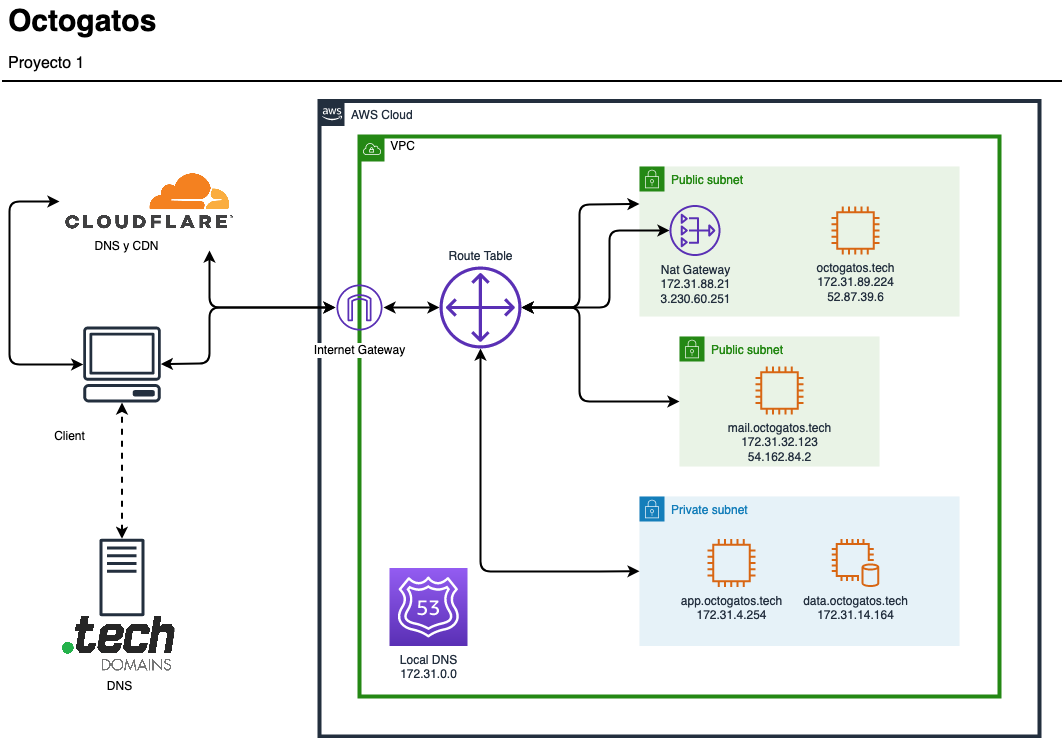
\includegraphics[width=\textwidth]{images/diagrama}
  \caption{Diagrama de configuraci\'on.}
  \label{fig:diagrama}
\end{figure}


%%%%%%%%%%%%%%%%%%%%%%%%%%%%%%%%%%%%%%%%%%%%%%%%%%%%%%%%%%%%%%%%
%%%%%%%%%%%%%%%%%%%%%%%%%%%%%%%%%%%%%%%%%%%%%%%%%%%%%%%%%%%%%%%%
%%%%%%%%%%%%%%%%%%%%%%%%%%%%%%%%%%%%%%%%%%%%%%%%%%%%%%%%%%%%%%%%
%%%%%%%%%%%%%%%%%%%%%%%%               %%%%%%%%%%%%%%%%%%%%%%%%%
%%%%%%%%%%%%%%%%%%%%%%%%%%%%%%%%%%%%%%%%%%%%%%%%%%%%%%%%%%%%%%%%
%%%%%%%%%%%%%%%%%%%%%%%%%%%%%%%%%%%%%%%%%%%%%%%%%%%%%%%%%%%%%%%%
%%%%%%%%%%%%%%%%%%%%%%%%%%%%%%%%%%%%%%%%%%%%%%%%%%%%%%%%%%%%%%%%


\section{Direcciones IPv6}

Las instancias correspondientes al servidor web y al
servidor de correo electr\'onico cuentan con direcciones
IPv6.   Para asignarle una direcci\'on IPv6 a nuestras
instancias se llevaron a cabo los siguientes pasos.
\begin{enumerate}
  \item Asociar un bloque CIDR IPv6 a nuestra VPC y
    subredes.

  \item Actualizar las tablas de enrutamiento.

  \item Actualizar los grupos de seguridad.

  \item Asignar direcciones IPv6 a las instancias.
\end{enumerate}

No ahondaremos en las instrucciones precisas para estos
pasos, pues pueden consultarse en el documento de AWS
que se encuentra en \href{https://docs.aws.amazon.com/vpc/latest/userguide/vpc-migrate-ipv6.html}{esta liga}.  Sin embargo,
creemos valioso mencionar que, aunque en el Paso 3 diga
que las reglas de ACL se configuran autom\'aticamente,
nosotros tuvimos que hacerlo a mano.

%%%%%%%%%%%%%%%%%%%%%%%%%%%%%%%%%%%%%%%%%%%%%%%%%%%%%%%%%%%%%%%%
%%%%%%%%%%%%%%%%%%%%%%%%%%%%%%%%%%%%%%%%%%%%%%%%%%%%%%%%%%%%%%%%
%%%%%%%%%%%%%%%%%%%%%%%%%%%%%%%%%%%%%%%%%%%%%%%%%%%%%%%%%%%%%%%%
%%%%%%%%%%%%%%%%%%%%%%%%               %%%%%%%%%%%%%%%%%%%%%%%%%
%%%%%%%%%%%%%%%%%%%%%%%%%%%%%%%%%%%%%%%%%%%%%%%%%%%%%%%%%%%%%%%%
%%%%%%%%%%%%%%%%%%%%%%%%%%%%%%%%%%%%%%%%%%%%%%%%%%%%%%%%%%%%%%%%
%%%%%%%%%%%%%%%%%%%%%%%%%%%%%%%%%%%%%%%%%%%%%%%%%%%%%%%%%%%%%%%%


\section{Registros DNS}
\label{sec:dns}

Para realizar esta configuraci\'on, fue necesario
actualizar los name servers de nuestro dominio,
para que usara los name servers de Cloudflare,
esto se configur\'o en el panel de control de
\href{https://get.tech}{get.tech}, bajo la opci\'on
``Name Servers''.   La configuraci\'on puede
verse en la Figura \ref{fig:nameServers}.
\begin{figure}[H]
  \centering
  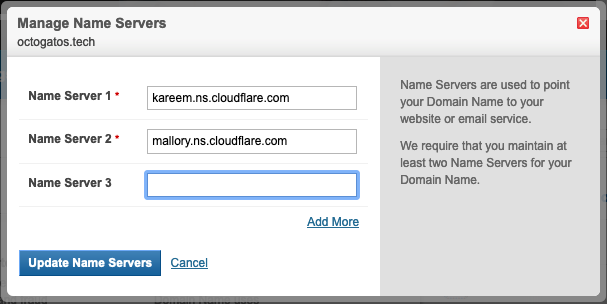
\includegraphics[width=0.7\textwidth]{DNS/nameServers}
  \caption{Configuraci\'on de los name servers para
           nuestro dominio.}
  \label{fig:nameServers}
\end{figure}

Se configuraron los siguiente registros DNS
externos en Cloudflare.
\begin{enumerate}
  \item A (Web Server - octogatos.tech - 52.87.39.6).

  \item A (Email Server - mail.octogatos.tech - 54.162.84.2).

  \item A (Email Server - postfixadmin.mail.octogatos.tech
                        - 54.162.84.2).

  \item AAAA (Web Server - octogatos.tech
                         - 2600:1f18:22c6:b16:1e05:b4d5:f19:61d).

  \item AAAA (Email Server - mail.octogatos.tech
                           - 2600:1f18:22c6:b00:9ca8:5c2a:c3c:d17f).

  \item CNAME (Web Server - www.octogatos.tech).

  \item MX (Web Server - 10 mail.octogatos.tech).

  \item TXT (Email Server - SPF).

  \item TXT (Email Server - DKIM).

  \item TXT (Email Server - DMARC).
\end{enumerate}
En la Figura \ref{fig:dnsExterno} se muestra la
evidencia respecto a esta configuraci\'on, misma
que puede ser verificada con el comando \ttt{dig},
salvo por aquellos registros para los que el proxy
de Cloudflare est\'a activo.
\begin{figure}[H]
  \centering
  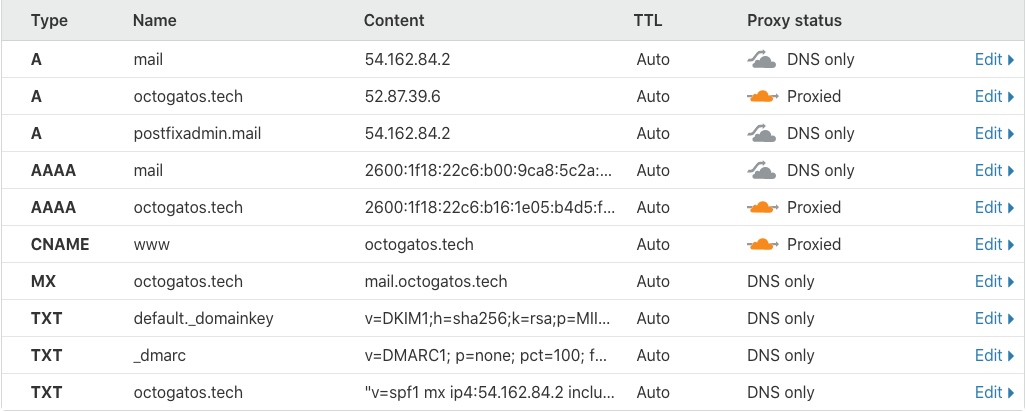
\includegraphics[width=0.85\textwidth]{DNS/dnsExterno}
  \caption{Configuraci\'on de los registros DNS externos.}
  \label{fig:dnsExterno}
\end{figure}

Adicionalmente, se configur\'o el registro PTR para
el servidor de correo, mediante la solicitud a Amazon
para abrir el puerto 25.

Se utiliz\'o Route 53 para configurar algunos registros
internos.   Para este fin, primero creamos una
``private hosted zone'', siguiendo las instrucciones
que aparecen en
\href{https://docs.aws.amazon.com/Route53/latest/DeveloperGuide/hosted-zone-private-creating.html}{esta liga} (recurso
de AWS).   Para crear esta zona, simplemente elegimos
la opci\'on ``Create hosted zone'', elegimos el
nombre de dominio ``octogatos.tech'', y la VPC en la
que estamos trabajando para asociar a nuestra nueva
zona. Una vez creada, es posible iniciar la configuraci\'on
de registros, que es semejante a la que se har\'ia
usualmente con un DNS externo, pero se utilizan las
direcciones IP privadas.   Un ejemplo de configuraci\'on
se puede ver en la Figura \ref{fig:defineRecord}, donde
el tipo de registro que se eligi\'o fue ``Simple'' (se
asocia el nombre de dominio con una \'unica direcci\'on
IP).

\begin{figure}[H]
  \centering
  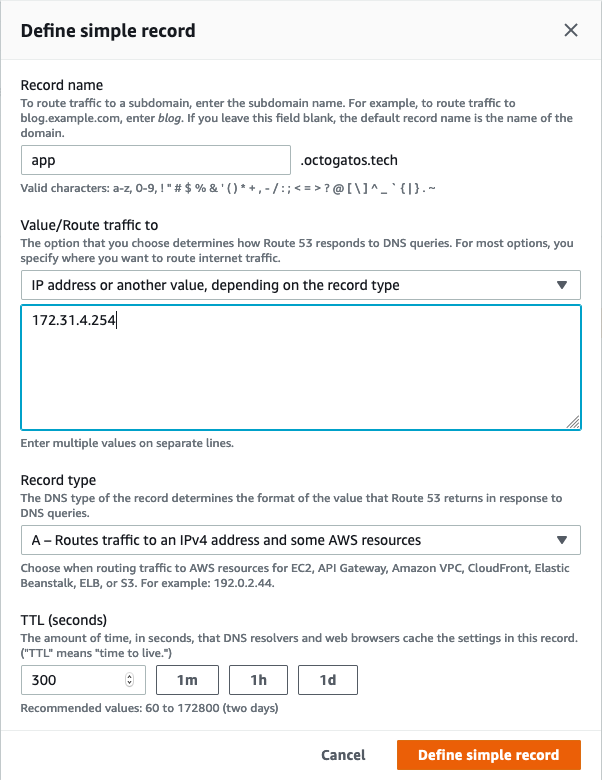
\includegraphics[width=0.38\textwidth]{DNS/defineRecord}
  \caption{Configuraci\'on del registro DNS interno para el
           app server usando Route 53.}
  \label{fig:defineRecord}
\end{figure}

Es posible configurar y crear m\'ultiples registros
a la vez, como se muestra en la Figura
\ref{fig:createRecord}

\begin{figure}[H]
  \centering
  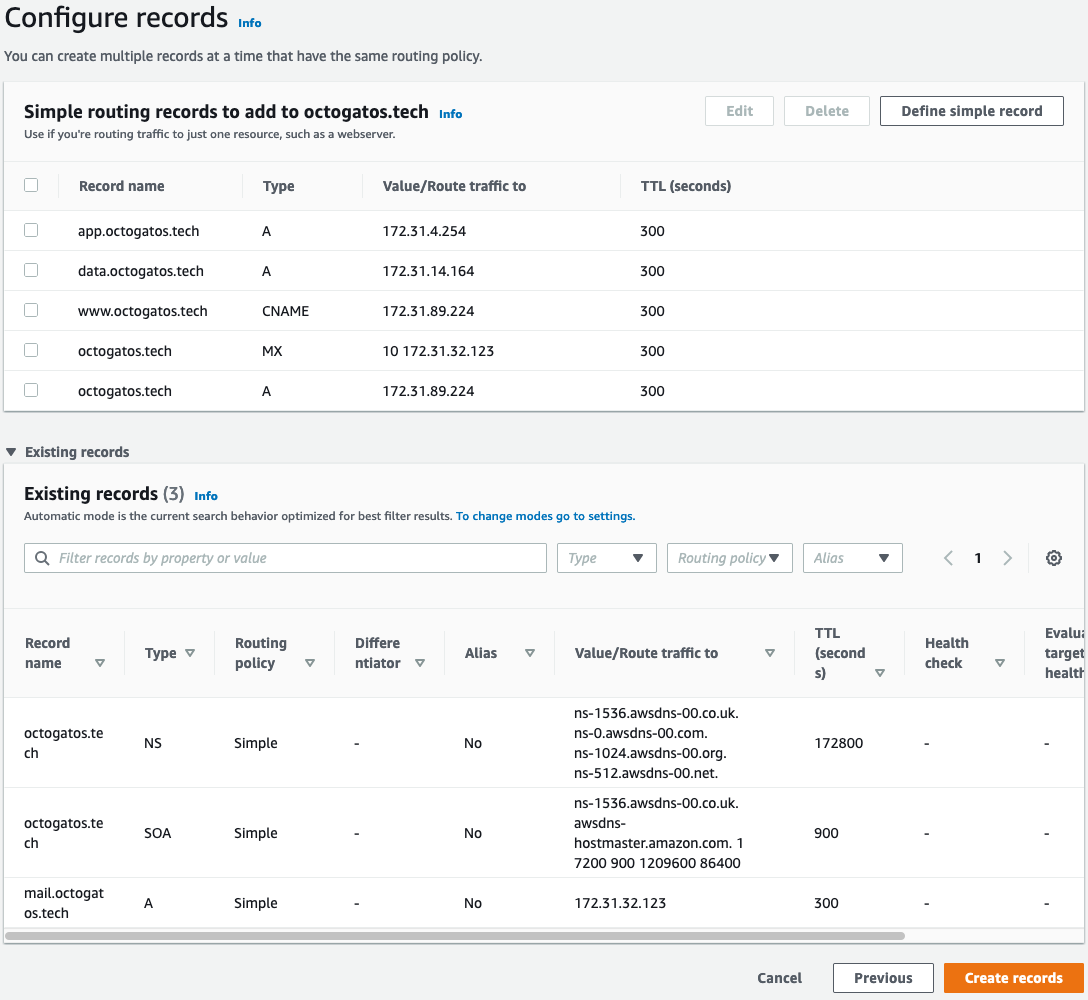
\includegraphics[width=0.8\textwidth]{DNS/createRecord}
  \caption{Creaci\'on de m\'ultiples registros DNS internos
           en Route 53.}
  \label{fig:createRecord}
\end{figure}


Usando Route 53, se configuraron los siguientes
registros internos.
\begin{enumerate}
  \item A (Web Server - octogatos.tech - 172.31.89.224).

  \item A (Email Server - mail.octogatos.tech - 172.31.32.123).

  \item A (App Server - app.octogatos.tech - 172.31.4.254).

  \item A (Data Server - data.octogatos.tech - 172.31.14.164).

  \item CNAME (Web Server - www.octogatos.tech).

  \item MX (Web Server - 10 172.31.32.123).
\end{enumerate}
La evidencia de esta configuraci\'on se muestra en
la Figura \ref{fig:createdRecord}
\begin{figure}[H]
  \centering
  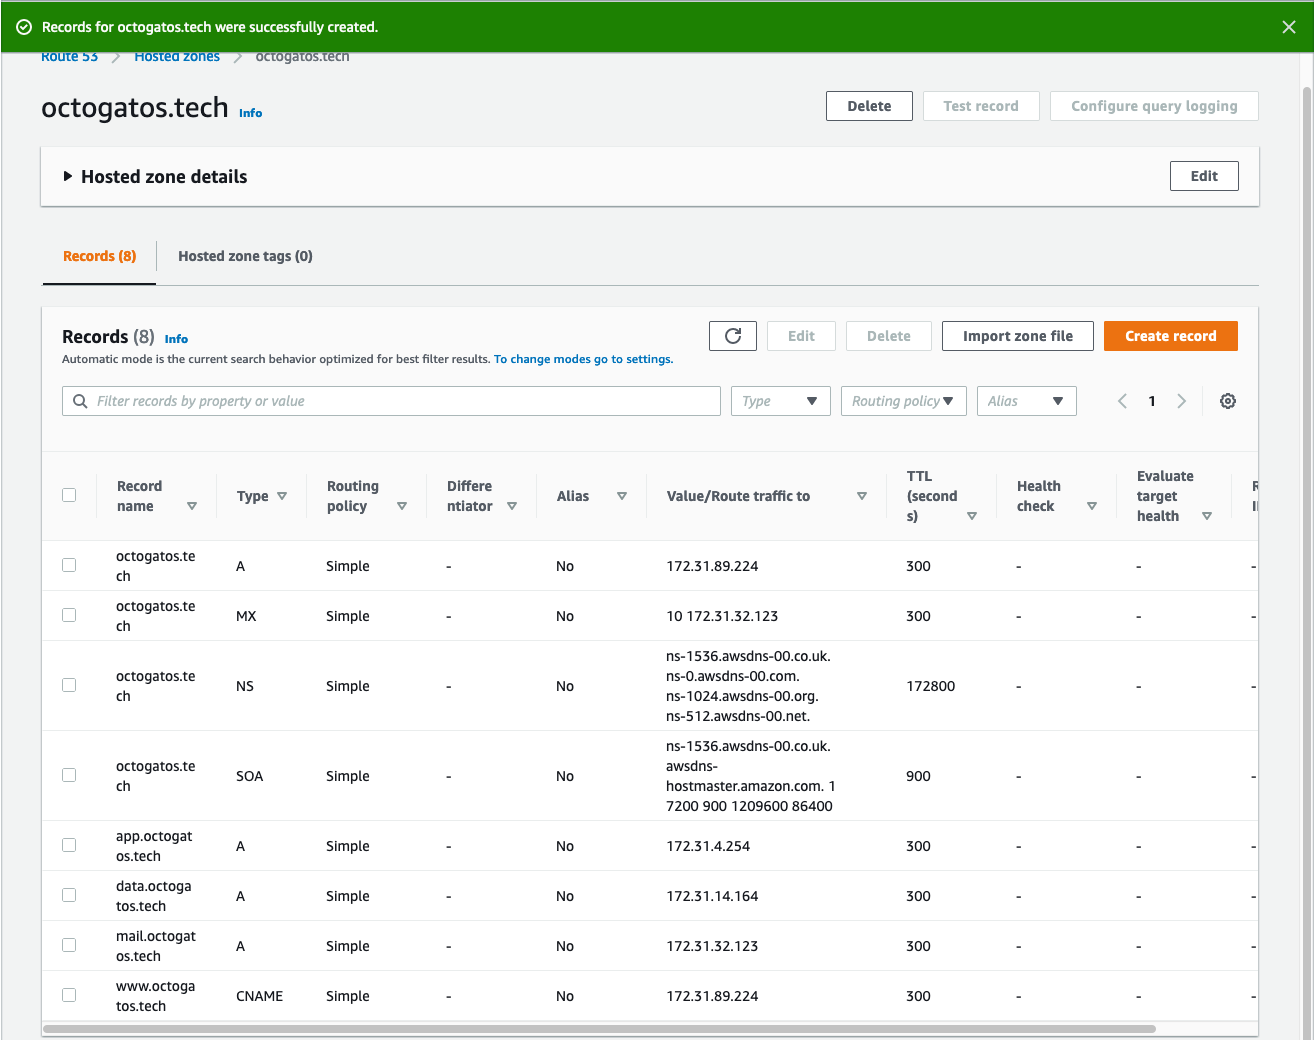
\includegraphics[width=0.9\textwidth]{DNS/createdRecord}
  \caption{Registros DNS internos configurados en Route 53.}
  \label{fig:createdRecord}
\end{figure}

%%%%%%%%%%%%%%%%%%%%%%%%%%%%%%%%%%%%%%%%%%%%%%%%%%%%%%%%%%%%%%%%
%%%%%%%%%%%%%%%%%%%%%%%%%%%%%%%%%%%%%%%%%%%%%%%%%%%%%%%%%%%%%%%%
%%%%%%%%%%%%%%%%%%%%%%%%%%%%%%%%%%%%%%%%%%%%%%%%%%%%%%%%%%%%%%%%
%%%%%%%%%%%%%%%%%%%%%%%%               %%%%%%%%%%%%%%%%%%%%%%%%%
%%%%%%%%%%%%%%%%%%%%%%%%%%%%%%%%%%%%%%%%%%%%%%%%%%%%%%%%%%%%%%%%
%%%%%%%%%%%%%%%%%%%%%%%%%%%%%%%%%%%%%%%%%%%%%%%%%%%%%%%%%%%%%%%%
%%%%%%%%%%%%%%%%%%%%%%%%%%%%%%%%%%%%%%%%%%%%%%%%%%%%%%%%%%%%%%%%


\section{Cloudflare}

Se utilaron tres servicios de
\href{https://www.cloudflare.com/}{Cloudflare}, a saber,
su DNS, como una capa de seguridad adicional entre el
usuario y el proxy de Cloudflare, y como Red de
Distribuci\'on de Contenidos (CDN).

Respecto a su uso como DNS, ya se habl\'o de la
configuraci\'on en la Secci\'on \ref{sec:dns}.   Para
su uso como CDN, configuramos dos reglas de CDN, una
para servir hojas de estilo (CSS) y otra para servir
im\'agenes.   Para la configuraci\'on simplemente
elegimos la regla de cach\'e y el recurso que queremos
que sea servido por Cloudflare.   En nuestro caso,
elegimos Edge Cache TTL, que nos permite indicar
un tiempo que, al transcurrir, Cloudflare solicitar\'a
una actualizaci\'on del recurso.   La configuraci\'on
de ambas reglas puede verse en la Figura
\ref{fig:pageRules}.

\begin{figure}[H]
  \centering
  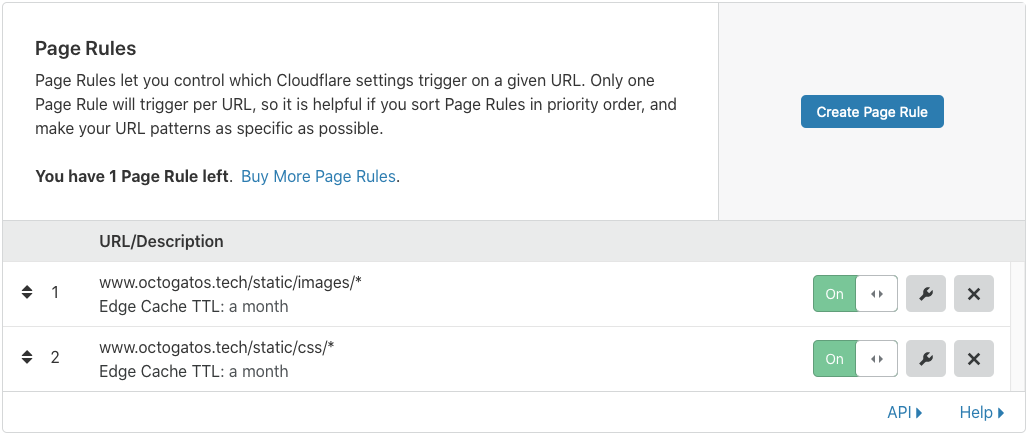
\includegraphics[width=0.8\textwidth]{cloudflare/pageRules}
  \caption{Configuraci\'on de page rules en Cloudflare.}
  \label{fig:pageRules}
\end{figure}

Para ver que estas reglas realmente est\'an funcionando,
podemos elegir la opci\'on ``Inspeccionar Elemento'' en
nuestra p\'agina \href{https://octogatos.tech}{octogatos.tech},
y notar que el valor \ttt{cf-cache-status} asociado a
a la imagen jazzCats.jpg es \ttt{HIT}, lo que significa que
fue encontrado al buscarse en el cache ofrecido por Cloudflare.
Puede notarse adem\'as que el valor de \ttt{server} es
cloudflare (Figura \ref{fig:pageRulesHit}).

% ALERT
% Actualizar el SS por uno que no tenga un 404

\begin{figure}[H]
  \centering
  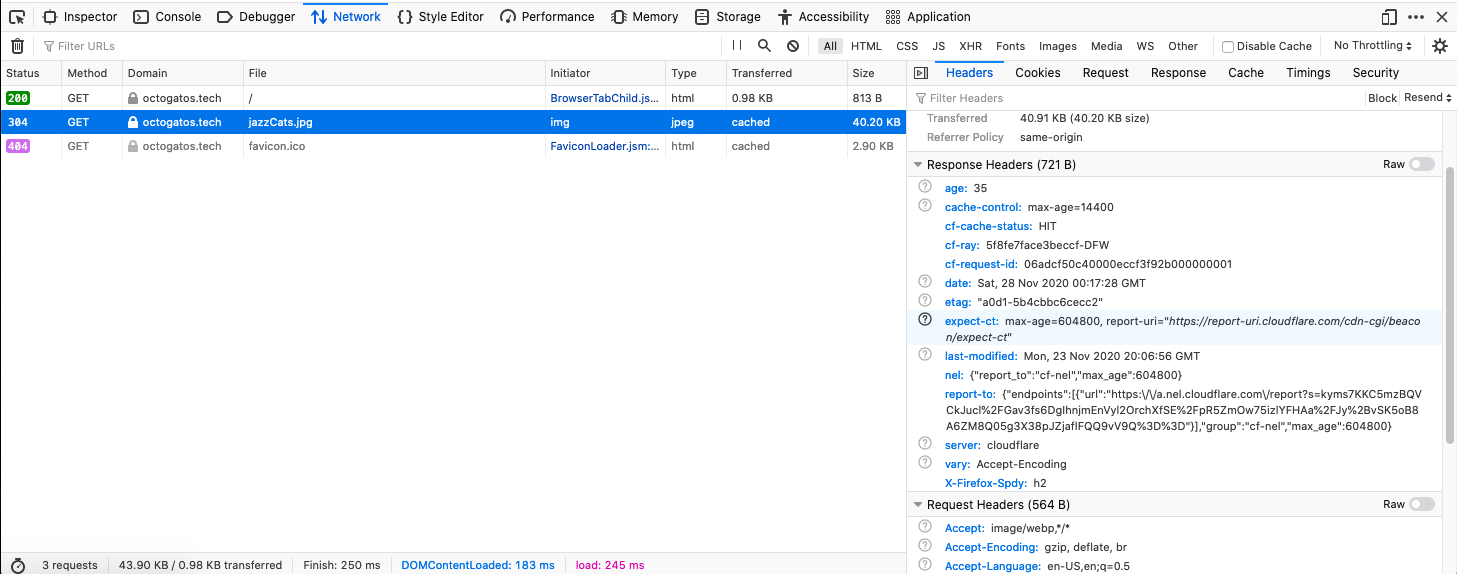
\includegraphics[width=\textwidth]{cloudflare/pageRulesHit}
  \caption{Configuraci\'on de page rules en Cloudflare.}
  \label{fig:pageRulesHit}
\end{figure}

Por otro lado, el modo de encriptaci\'on que se
configur\'o en Cloudflare es Completo (estricto).
Como ya se mencion\'o, Cloudflare ofrece la
encriptaci\'on entre el usuario final y sus
servidores (que estamos usando como proxies),
y nuestros certificados de Let's Encrypt proporcionan
la seguridad entre los servidores de Cloudflare
y nuestro servidor en AWS.   El estado actual de
la configuraci\'on de SSL/TLS puede verse en la
Figura \ref{fig:cfEncryption}.

\begin{figure}[H]
  \centering
  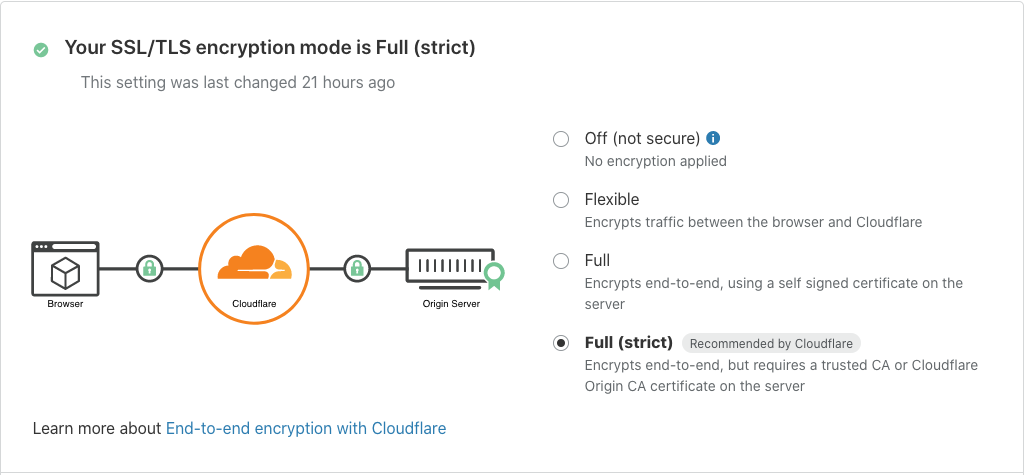
\includegraphics[width=\textwidth]{cloudflare/cfEncryption}
  \caption{Configuraci\'on de SSL/TLS en Cloudflare.}
  \label{fig:cfEncryption}
\end{figure}


%%%%%%%%%%%%%%%%%%%%%%%%%%%%%%%%%%%%%%%%%%%%%%%%%%%%%%%%%%%%%%%%
%%%%%%%%%%%%%%%%%%%%%%%%%%%%%%%%%%%%%%%%%%%%%%%%%%%%%%%%%%%%%%%%
%%%%%%%%%%%%%%%%%%%%%%%%%%%%%%%%%%%%%%%%%%%%%%%%%%%%%%%%%%%%%%%%
%%%%%%%%%%%%%%%%%%%%%%%%               %%%%%%%%%%%%%%%%%%%%%%%%%
%%%%%%%%%%%%%%%%%%%%%%%%%%%%%%%%%%%%%%%%%%%%%%%%%%%%%%%%%%%%%%%%
%%%%%%%%%%%%%%%%%%%%%%%%%%%%%%%%%%%%%%%%%%%%%%%%%%%%%%%%%%%%%%%%
%%%%%%%%%%%%%%%%%%%%%%%%%%%%%%%%%%%%%%%%%%%%%%%%%%%%%%%%%%%%%%%%


\section{Web Server}

Para nuestro Web Server utilizamos la instancia EC2 que
fue creada en la Pr\'actica 2, por lo que no ahondaremos
en detalles respecto a su creaci\'on.   Es importante
recalcar que tambi\'en reutilizamos el certificado
expedido por \href{https://letsencrypt.org/}{Let's Encrypt},
y configurado con \href{https://certbot.eff.org/}{Certbot},
as\'i como la direcci\'on IP el\'astica de la Pr\'actica 2,
por lo que la configuraci\'on de la instancia en AWS se ve
como en la Figura \ref{fig:web-instancia}.

\begin{figure}[H]
  \centering
  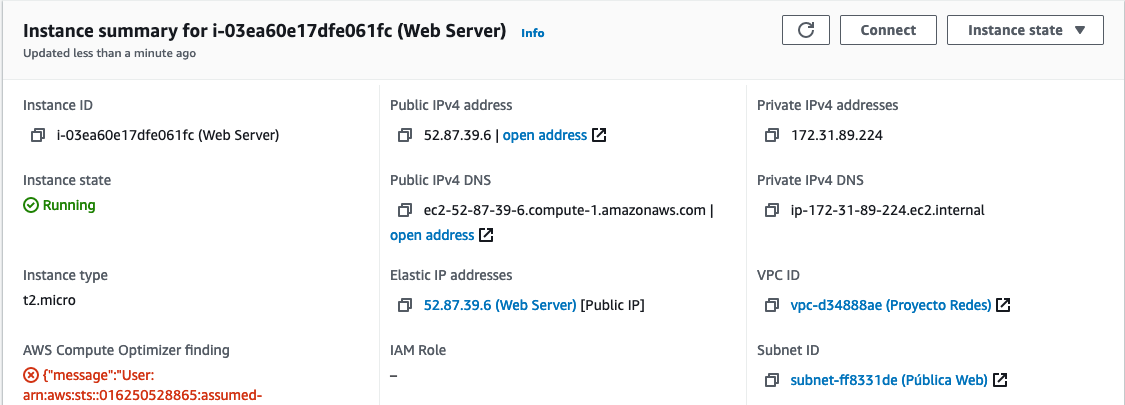
\includegraphics[width=\textwidth]{web/instancia}
  \caption{Configuraci\'on de la instancia del Web Server
           en AWS.}
  \label{fig:web-instancia}
\end{figure}

Como se puede ver en la figura, esta instancia se
encuentra en una subred, identificada con el nombre
``P\'ublica Web'', cuya configuraci\'on se muestra
en la figura \ref{fig:web-subred}.

\begin{figure}[H]
  \centering
  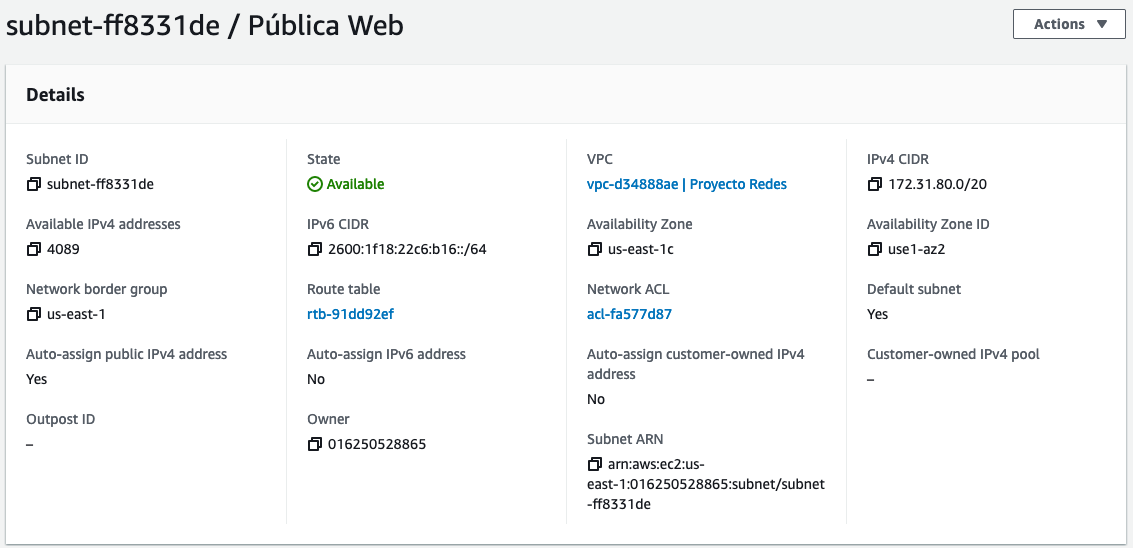
\includegraphics[width=\textwidth]{web/subred}
  \caption{Configuraci\'on de la primera subred p\'ublica.}
  \label{fig:web-subred}
\end{figure}

Adem\'as, esta instancia cuenta con una direcci\'on IPv6,
misma que puede verse en la configuraci\'on de red de la
instancia, misma que puede apreciarse en la Figura
\ref{fig:web-ipv6}.   N\'otese que la direcci\'on IPv6
de esta instancia efectivamente coincide con la que se
asign\'o a la subred correspondiente.

\begin{figure}[H]
  \centering
  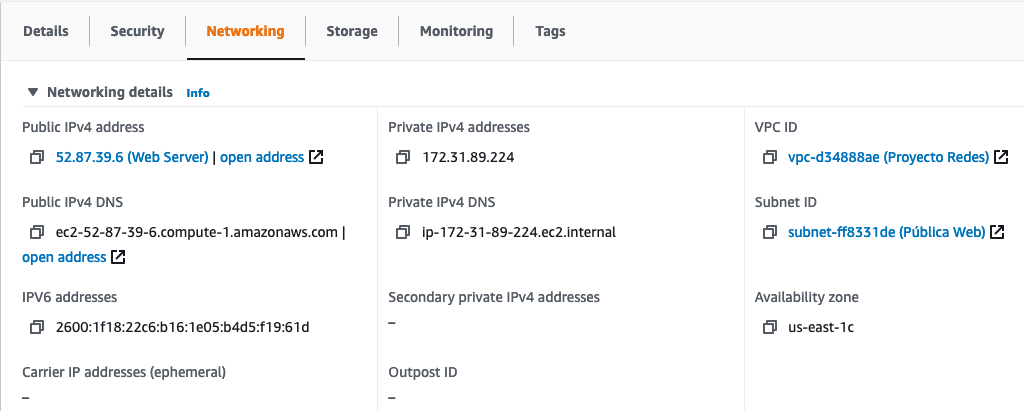
\includegraphics[width=\textwidth]{web/ipv6}
  \caption{Configuraci\'on de red del servidor web.}
  \label{fig:web-ipv6}
\end{figure}

Nuestro servidor web act\'ua principalmente como
forward y reverse proxy.   Esta opci\'on se habilita
como parte de la configuraci\'on del servidor Apache.
Hay varios recursos en internet sobre c\'omo realizar
esta configuraci\'on paso a paso, por ejemplo, es
posible seguir las instrucciones dadas por
\href{https://www.digitalocean.com/community/tutorials/how-to-use-apache-http-server-as-reverse-proxy-using-mod_proxy-extension}{este
tutorial} de Digital Ocean.   Para llevar a cabo,
la configuraci\'on, primero es necesario activar
algunos m\'odulos de apache, lo que puede hacerse
con los comandos
\begin{lstlisting}
$ sudo a2enmod proxy
$ sudo a2enmod proxy_http
$ sudo a2enmod rewrite
$ sudo a2enmos proxy_connect
$ sudo a2enmod proxy_html
\end{lstlisting}

Existe la posibilidad de que el m\'odulo no est\'e
instalado, en cuyo caso puede instalarse con el
comando
\begin{lstlisting}
sudo apt install -y libapache2-mod-proxy-html libxml2-dev
\end{lstlisting}

Una vez habilitados estos m\'odulos, procedemos
a actualizar la configuraci\'on del servidor
Apache, con el comando
\begin{lstlisting}
sudo vi /etc/apache2/sites-available/redesfc.conf
\end{lstlisting}

Tambi\'en es necesario actualizar la configuraci\'on
creada por Certbot cuando obtuvimos el certificado
de Let's Encrypt, para el virtual host de HTTPS en
el puerto 443, lo que puede hacerse con el siguiente
comando
\begin{lstlisting}
sudo vi /etc/apache2/sites-available/redesfc-le-ssl.conf
\end{lstlisting}

Las configuraciones deben de verse como en la
Figura \ref{fig:web-mapache}.
\begin{figure}[H]
  \centering
  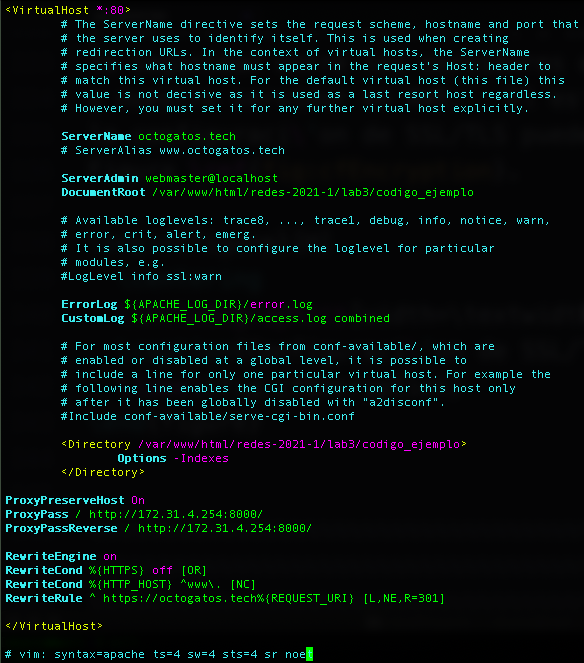
\includegraphics[width=0.45\textwidth]{web/mapache80}
  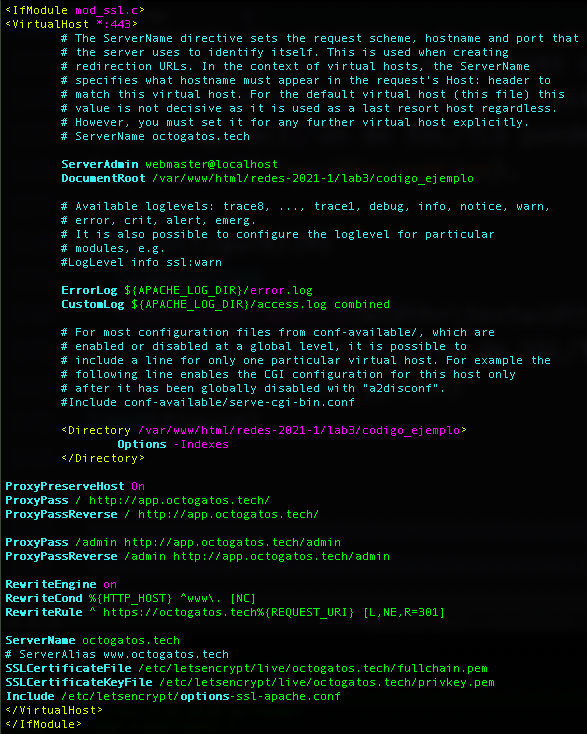
\includegraphics[width=0.45\textwidth]{web/mapache443}
  \caption{Configuraci\'on del servidor Apache como proxy.}
  \label{fig:web-mapache}
\end{figure}

Las l\'ineas que nos interesan son aquellas que empiezan
con la palabra ``Proxy'', en donde se activa la opci\'on
\ttt{ProxyPreserveHost}, que indica a Apache que debe
mantener la direcci\'on url del host que actua como proxy,
y las opciones \ttt{ProxyPass} y \ttt{ProxyReverse}, que
indican a Apache que redireccione las peticiones hacia y
desde el servidor al que est\'a sirviendo como proxy (en
nuestro caso, el servidor de aplicaci\'on).

En las misma figura es posible notar que tenemos
la l\'inea \ttt{Options -Indexes}, que deshabilita
la opci\'on de enlistar los contenidos de las carpetas
que se encuentran en nuestro directorio ra\'iz.

Adicionalmente, y tambi\'en en la Figura \ref{fig:web-mapache},
es posible encontrar algunas l\'ineas que empiezan con
la palabra ``Rewrite''.   La finalidad de estas es lograr
la redirecci\'on de
\href{http://octogatos.tech}{http://octogatos.tech},
\href{http://www.octogatos.tech}{http://www.octogatos.tech}, y
\href{https://www.octogatos.tech}{https://www.octogatos.tech}
a \href{https://octogatos.tech}{https://octogatos.tech}.




%%%%%%%%%%%%%%%%%%%%%%%%%%%%%%%%%%%%%%%%%%%%%%%%%%%%%%%%%%%%%%%%
%%%%%%%%%%%%%%%%%%%%%%%%%%%%%%%%%%%%%%%%%%%%%%%%%%%%%%%%%%%%%%%%
%%%%%%%%%%%%%%%%%%%%%%%%%%%%%%%%%%%%%%%%%%%%%%%%%%%%%%%%%%%%%%%%
%%%%%%%%%%%%%%%%%%%%%%%%               %%%%%%%%%%%%%%%%%%%%%%%%%
%%%%%%%%%%%%%%%%%%%%%%%%%%%%%%%%%%%%%%%%%%%%%%%%%%%%%%%%%%%%%%%%
%%%%%%%%%%%%%%%%%%%%%%%%%%%%%%%%%%%%%%%%%%%%%%%%%%%%%%%%%%%%%%%%
%%%%%%%%%%%%%%%%%%%%%%%%%%%%%%%%%%%%%%%%%%%%%%%%%%%%%%%%%%%%%%%%


\section{Data Server}

Para la configuración inicial del data server, lo primordial
es tener instalado y configurado el manejador de base de datos
dentro de nuestro servidor. Para ello optamos por Postgres
(12.5), el cual instalamos en nuestro servidor mediante el
comando:

\begin{lstlisting}
$ sudo apt install postgresql postgresql-contrib
\end{lstlisting}

\begin{figure}[H]
  \centering
  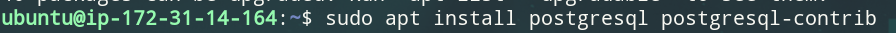
\includegraphics[width=\textwidth]{DATASERVER/exhibitA}
  \caption{Instalación de postgres en el data server.}
  \label{fig:DATASERVER-A}
\end{figure}

Como Postgres utiliza ``roles'' para manejar la autenticación y
autorización de creación de base de datos, es necesario acceder
al rol por omisión que crea Postgres para poder trabajar con su
manejador de base de datos. Accedemos al usuario por medio de:

\begin{lstlisting}
$ sudo -i -u postgres
\end{lstlisting}

Y ahora podemos acceder sin problema alguno a Postgres:

\begin{figure}[H]
  \centering
  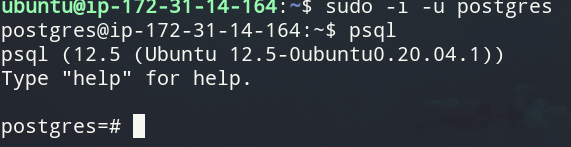
\includegraphics[width=0.8\textwidth]{DATASERVER/exhibitB}
  \caption{Manejador de Base de Datos Postgresql.}
  \label{fig:DATASERVER-B}
\end{figure}

Y creamos nuestra base de datos \ttt{octogatos} que va a ser
utilizada en este proyecto, en la que sólo el usuario
\ttt{postgres} va a poder acceder.

\begin{figure}[H]
  \centering
  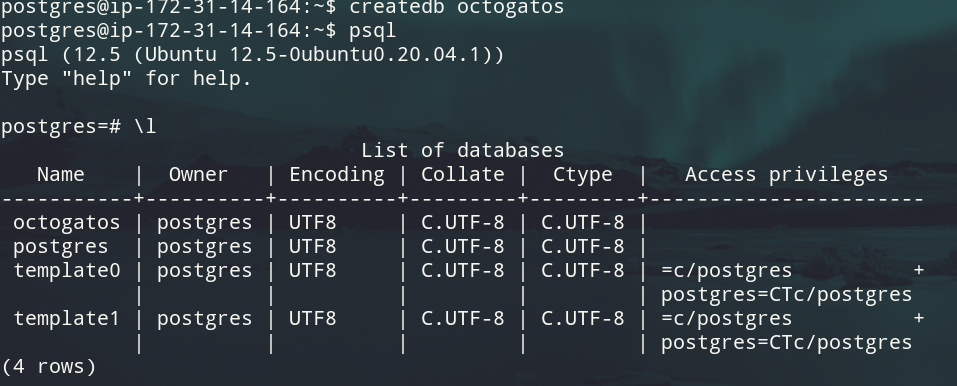
\includegraphics[width=0.9\textwidth]{DATASERVER/exhibitC}
  \caption{Creación de la base de datos del proyecto.}
  \label{fig:DATASERVER-C}
\end{figure}

Como sólo se podrá conectar la App Server a este servidor,
entonces es necesario indicar en la configuración que
confíamos solo vamos a confiar en las conexiones locales
(del mismo server a sí mismo) y en las conexiones que vengan
del App Server.

Para la conexión local, tenemos que modificar el archivo
\ttt{pg\_hba.conf}, sustituyendo la línea:

\begin{lstlisting}
local   all             postgres                                peer
\end{lstlisting}

Por la línea:
\begin{lstlisting}
local   all             postgres                                trust
\end{lstlisting}

Reiniciamos nuestro servidor y listo, ya se pueden ejecutar
\textit{scripts} de sql; por ejemplo creamos nuestra tabla
``user'':

\begin{figure}[H]
  \centering
  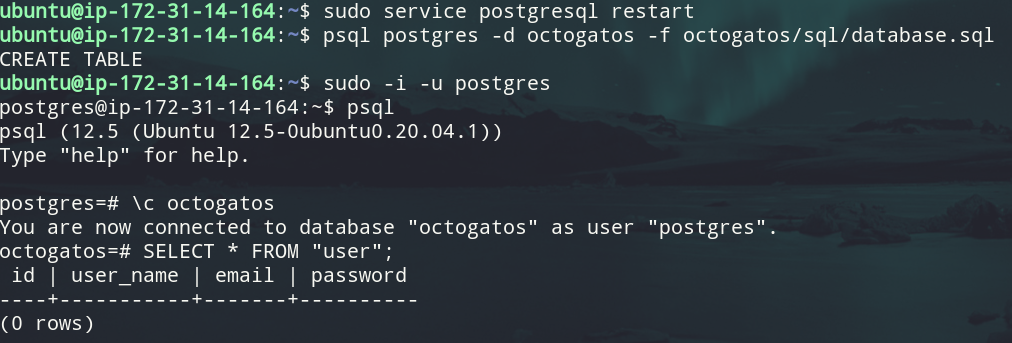
\includegraphics[width=0.9\textwidth]{DATASERVER/exhibitE}
  \caption{Creación de la tabla usuarios.}
  \label{fig:DATASERVER-E}
\end{figure}

Para la conexión remota, primero tenemos que verificar a qué
dirección IP se encuentra ligada el puerto 5432 (el puerto
que usa Postgres).

\begin{figure}[H]
  \centering
  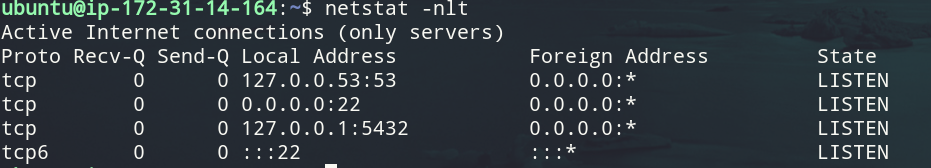
\includegraphics[width=0.9\textwidth]{DATASERVER/exhibitF}
  \caption{La dirección del puerto 5432.}
  \label{fig:DATASERVER-E}
\end{figure}

Si nosotros tratamos de conectarnos a este puerto, entonces no
vamos a tener éxito:

\begin{figure}[H]
  \centering
  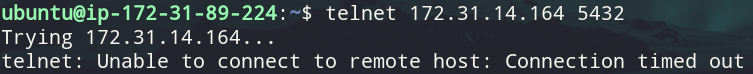
\includegraphics[width=0.9\textwidth]{DATASERVER/exhibitG}
  \caption{Primero intento de conexión al puerto 5432.}
  \label{fig:DATASERVER-G}
\end{figure}

Para poder resolver esto, necesitamos configurar nuestros
archivos \ttt{postgresql.conf} y \ttt{pg\_hba.conf}.
En el primer archivo cambiamos el valor de
\ttt{listen\_addresses} por:

\begin{lstlisting}
listen_addresses = '*'
\end{lstlisting}

Y también agregamos la dirección IP privada de la App
Server  al segundo archivo, para que sólo se pueda conectar
por medio del usuario \ttt{postgres} y con su contraseña:
\begin{lstlisting}
host    all             all              172.31.4.254/32                       md5
\end{lstlisting}

\begin{figure}[H]
  \centering
  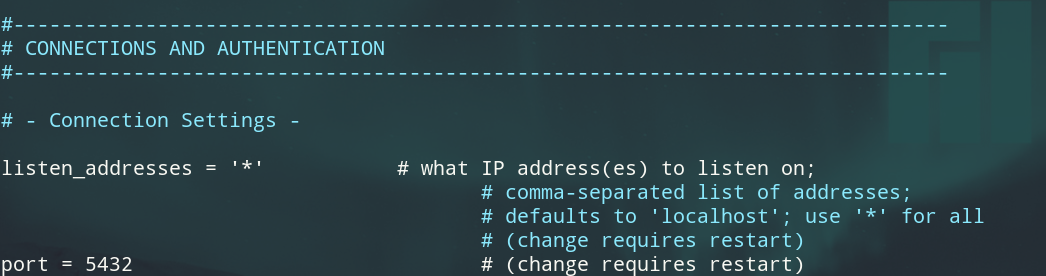
\includegraphics[width=0.9\textwidth]{DATASERVER/exhibitI}
  \label{fig:DATASERVER-I}
\end{figure}

\begin{figure}[H]
  \centering
  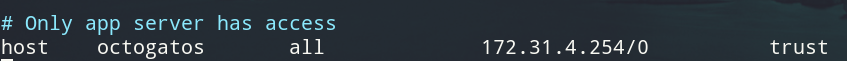
\includegraphics[width=0.9\textwidth]{DATASERVER/exhibitJ}
  \label{fig:DATASERVER-J}
\end{figure}

Sin embargo, si lo dejamos como lo tenemos ahorita, nuestro
servidor va a aceptar las conexiones de cualquier servidor,
por lo tanto tenemos que agregar este tipo de restricción
al \textit{security groups} de nuestro servidor.

\begin{figure}[H]
  \centering
  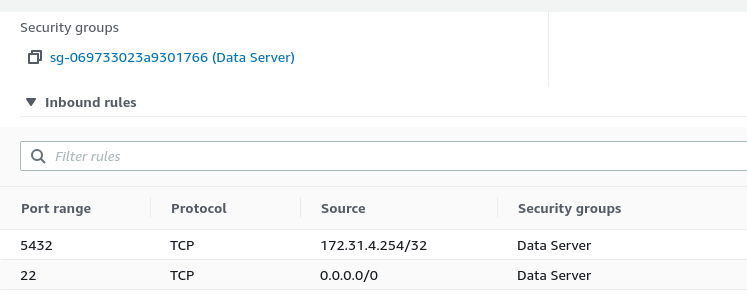
\includegraphics[width=0.9\textwidth]{DATASERVER/exhibitK}
  \label{fig:DATASERVER-K}
\end{figure}

Y listo, si accedemos a nuestro App Server y tratamos de
conectar a postgres, entonces vamos a tener éxito. Mientras
que si nos conectamos desde cualquier otro servidor o
dispositivo dentro de la red, entonces no se va a aceptar la
conexión.

\begin{figure}[H]
  \centering
  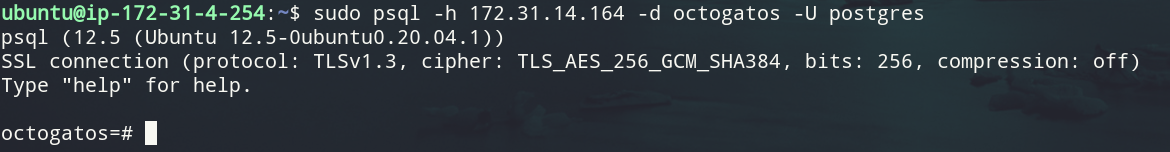
\includegraphics[width=0.9\textwidth]{DATASERVER/exhibitL}
  \caption{Intento exitoso para conectarse al Data Server desde la App Server.}
  \label{fig:DATASERVER-L}
\end{figure}

En la Figura \ref{fig:DATASERVER-L} tambi\'en se
puede observar que la conexi\'on se hacer con el protocolo
TLSv1.3, por lo que esta conexi\'on est\'a cifrada.


\section{Base De Datos}
Como se mencionó, para este proyecto se decidió utilizar
el marco de trabajo \textit{Django} pues nos facilita el
trabajo en múltiples áreas, una de ellas siendo la base
de datos y su uso para manejar las sesiones y los registros
de usuarios. Por este motivo, y por la utilidad de nuestro
proyecto, se decidió utilizar únicamente las tablas que crea
\textit{Django} por omisión. Así, el esquema de
nuestra base de datos se ve de la siguiente manera:

\begin{figure}[H]
  \centering
  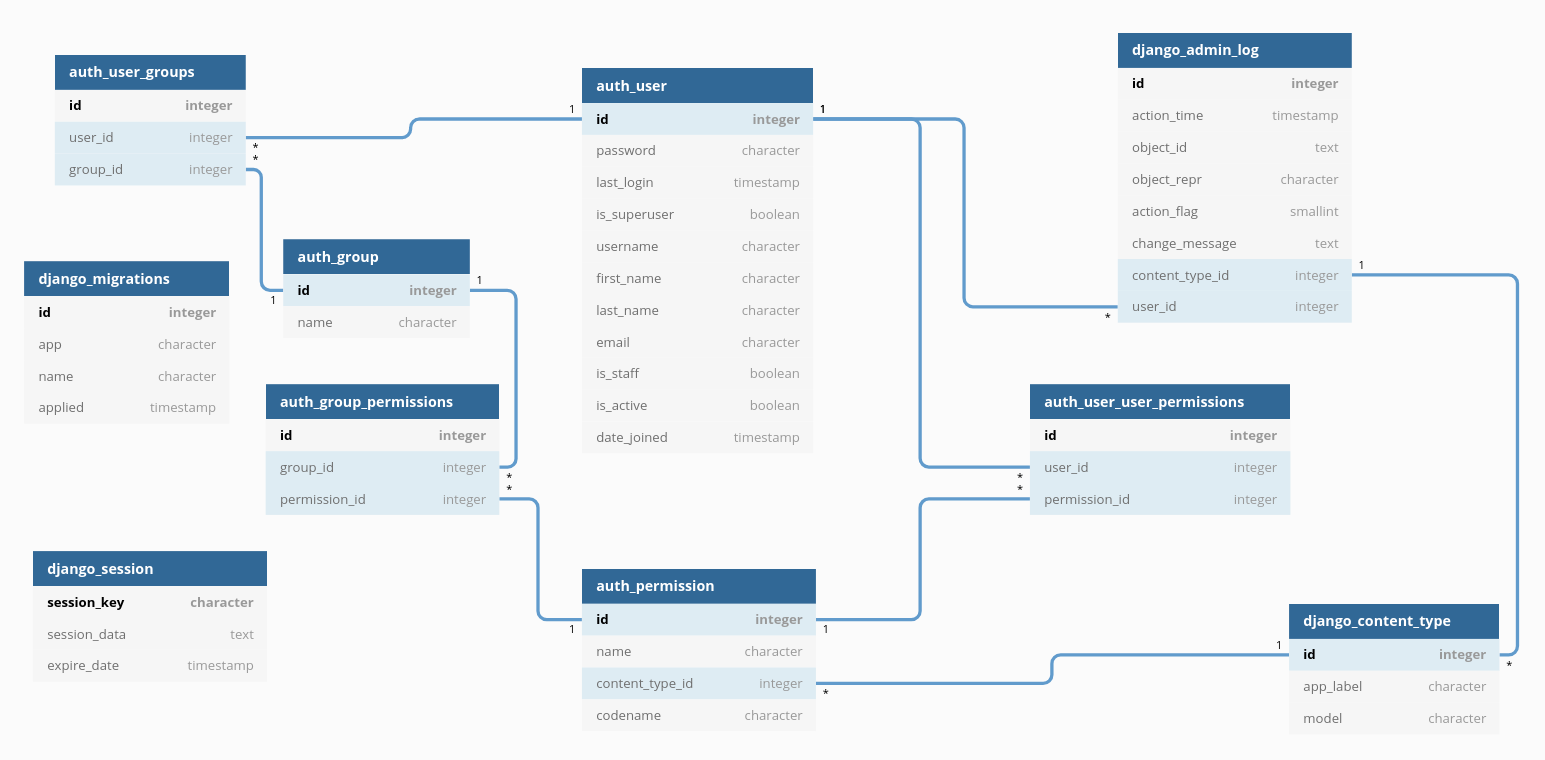
\includegraphics[width=0.8\textwidth]{BDD/diagram}
  \caption{ Diagrama de la base de datos}
\end{figure}

%%%%%%%%%%%%%%%%%%%%%%%%%%%%%%%%%%%%%%%%%%%%%%%%%%%%%%%%%%%%%%%%
%%%%%%%%%%%%%%%%%%%%%%%%%%%%%%%%%%%%%%%%%%%%%%%%%%%%%%%%%%%%%%%%
%%%%%%%%%%%%%%%%%%%%%%%%%%%%%%%%%%%%%%%%%%%%%%%%%%%%%%%%%%%%%%%%
%%%%%%%%%%%%%%%%%%%%%%%%               %%%%%%%%%%%%%%%%%%%%%%%%%
%%%%%%%%%%%%%%%%%%%%%%%%%%%%%%%%%%%%%%%%%%%%%%%%%%%%%%%%%%%%%%%%
%%%%%%%%%%%%%%%%%%%%%%%%%%%%%%%%%%%%%%%%%%%%%%%%%%%%%%%%%%%%%%%%
%%%%%%%%%%%%%%%%%%%%%%%%%%%%%%%%%%%%%%%%%%%%%%%%%%%%%%%%%%%%%%%%


\section{Email Server}

Para configurar el servidor de correo electr\'onico
utilizamos una instancia EC2 semejante a la que
se utiliz\'o para el servidor web.   Tambi\'en cuenta
con una direcci\'on IP el\'astica y con un certificado
emitido por \href{https://letsencrypt.org/}{Let's
Encrypt} que fue configurado en la instancia mediante
\href{https://certbot.eff.org/}{Certbot}.   Adem\'as
se utiliz\'o el subdominio \ttt{mail.octogatos.tech}
asociado a la IP el\'astica de esta instancia.   Es
posible verificar que el certificado funciona
correctamente entrando a
\href{https://mail.octogatos.tech/}{https://mail.octogatos.tech/}
y revisando el certificado en cualquier navegador.
La configuraci\'on de la instancia en AWS puede
revisarse en la Figura \ref{fig:email-instancia},
incluyendo la direcci\'on IPv6.

\begin{figure}[H]
  \centering
  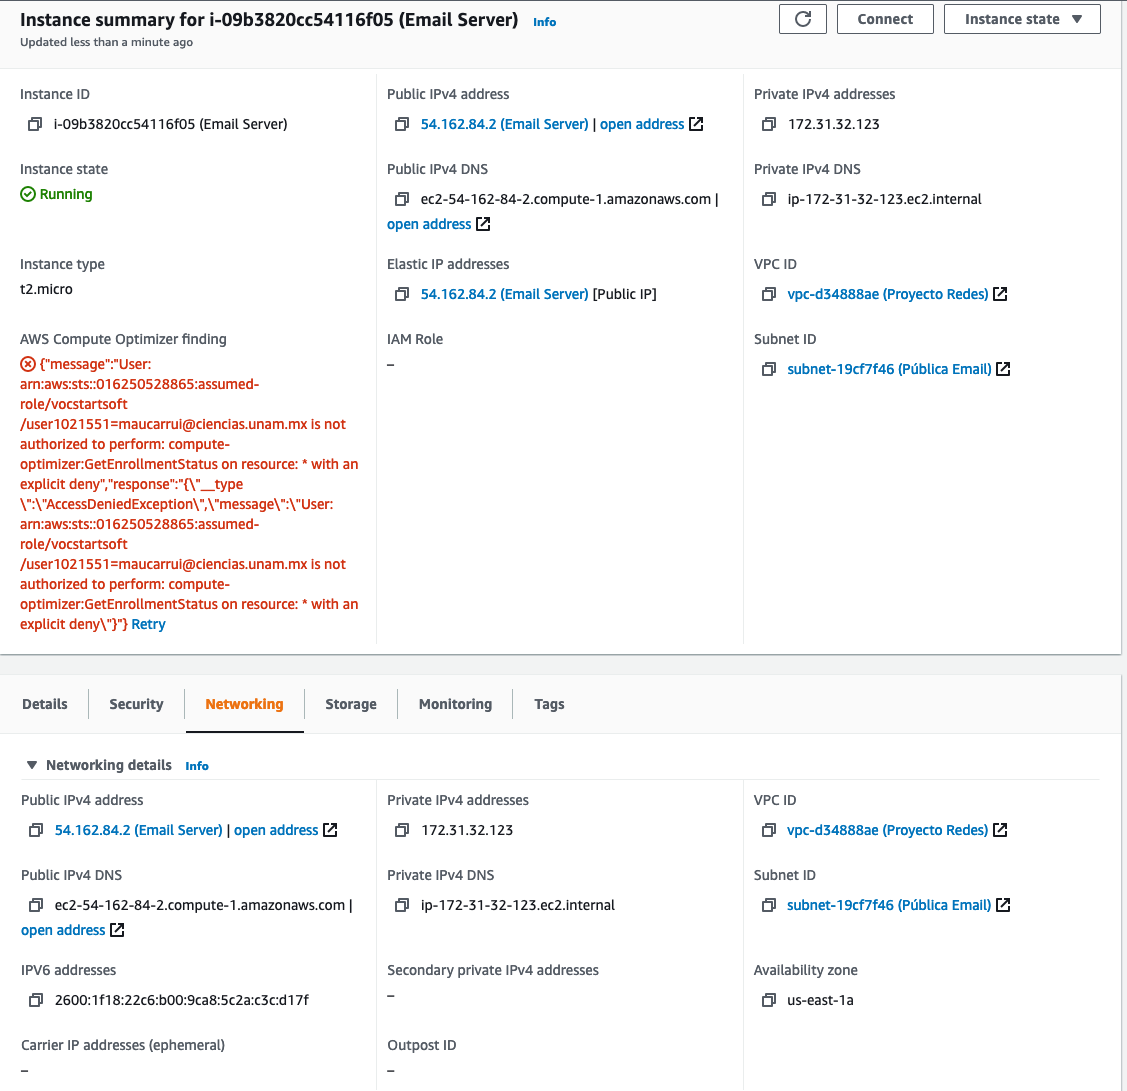
\includegraphics[width=0.9\textwidth]{email/instancia}
  \caption{Configuraci\'on EC2 del servidor de correo.}
  \label{fig:email-instancia}
\end{figure}

Como se mencion\'o en la Secci\'on \ref{sec:diagrama},
esta instancia cuenta con su propia subred p\'ublica,
cuya configuraci\'on puede verse en la Figura
\ref{fig:email-subred}.

\begin{figure}[H]
  \centering
  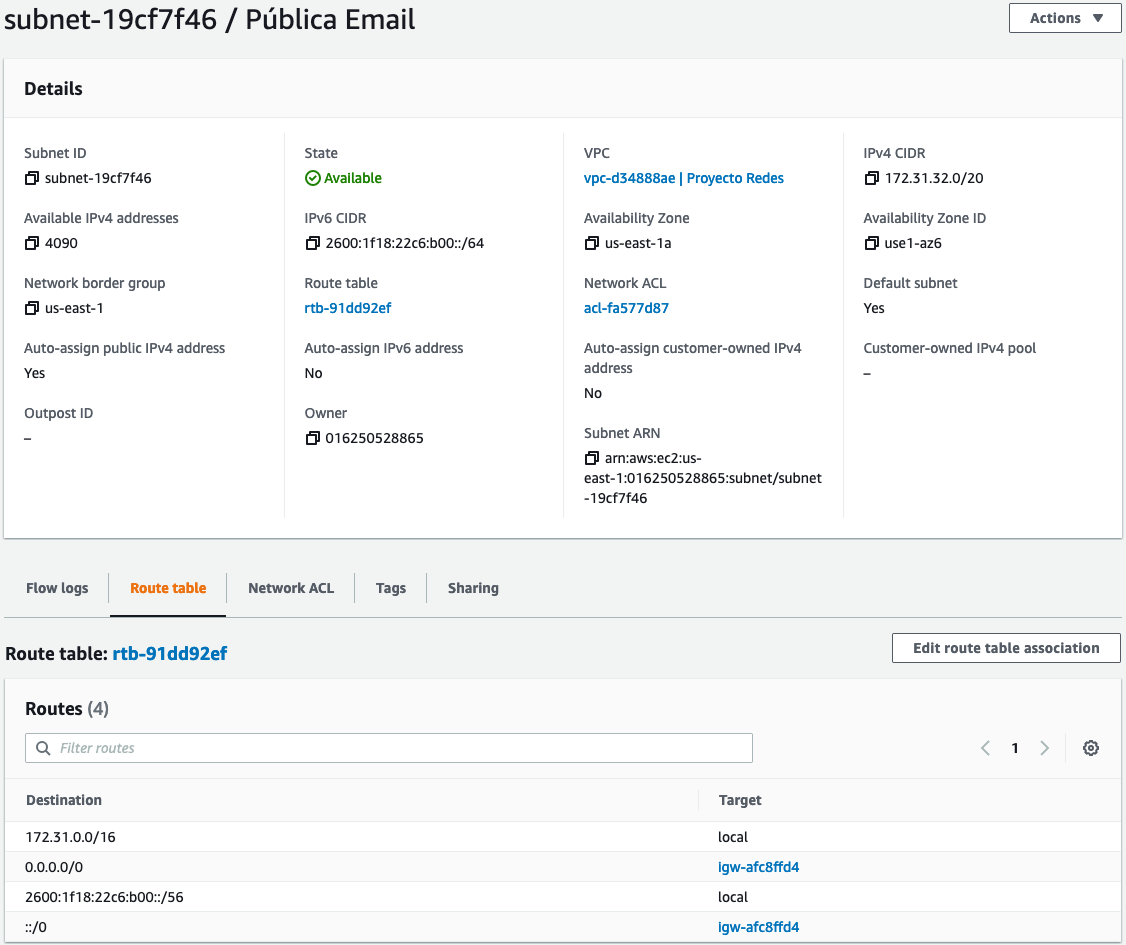
\includegraphics[width=0.9\textwidth]{email/subred}
  \caption{Configuraci\'on de la segunda subred p\'ublica.}
  \label{fig:email-subred}
\end{figure}

Adicionalmente, es necesario tener un grupo de
seguridad espec\'ifico para esta instancia, pues
es necesario tener abiertos varios puertos para
los distintos servicios que se van a ofrecer:
80 (HTTP para webmail), 110 (POP3), 995 (POP3S),
993 (IMAPS), 22 (SSH), 25 (SMTP), 143 (IMAP),
465 (SMTPS), 587 (SMTPS), 443 (HTTPS).   La
configuraci\'on de las reglas de entrada en este
grupo de seguridad pueden verse en la Figura
\ref{fig:email-seguridad}.

\begin{figure}[H]
  \centering
  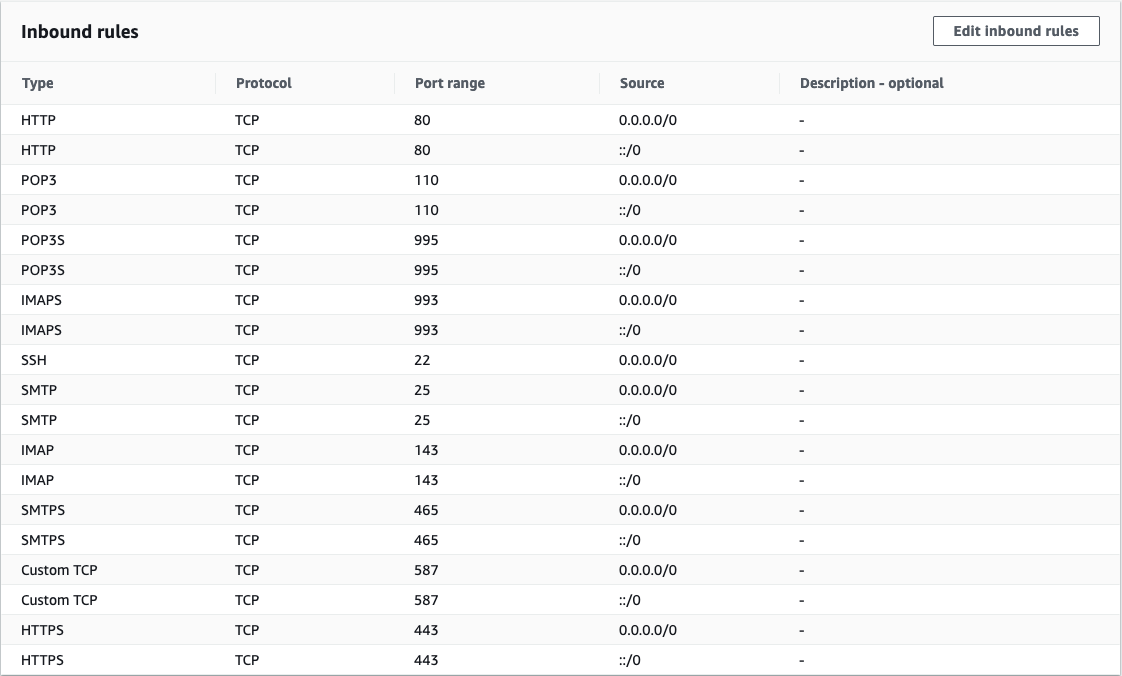
\includegraphics[width=0.9\textwidth]{email/seguridad}
  \caption{Configuraci\'on del grupo de seguridad para
           el servidor de correo.}
  \label{fig:email-seguridad}
\end{figure}

Para configurar el servidor de correo, se siguieron
los siguientes tutoriales:

\begin{enumerate}
  \item \href{https://www.linuxbabe.com/mail-server/setup-basic-postfix-mail-sever-ubuntu}{Build Your Own Email Server on Ubuntu: Basic Postfix Setup}

  \item \href{https://www.linuxbabe.com/mail-server/secure-email-server-ubuntu-postfix-dovecot}{Set up Dovecot IMAP server and TLS encryption}

  \item \href{https://www.linuxbabe.com/mail-server/postfixadmin-create-virtual-mailboxes-ubuntu-20-04}{Create Virtual Mailboxes with PostfixAdmin}

  \item \href{https://www.linuxbabe.com/mail-server/setting-up-dkim-and-spf}{Creating SPF and DKIM record to get through spam filters}

  \item \href{https://www.linuxbabe.com/mail-server/create-dmarc-record}{Setting Up DMARC to protect your domain reputation}
\end{enumerate}

Se utiliz\'o \href{http://www.postfix.org/}{Postfix} como
servidor SMTP.   Como prerrequisitos, se configur\'o el
nombre de dominio \ttt{mail.octogatos.tech}, y se cre\'o
un registro MX para \ttt{octogatos.tech} que apunta hacia
\ttt{mail.octogatos.tech}, adem\'as de registros \ttt{A},
\ttt{AAAA} y \ttt{PTR} para \ttt{mail.octogatos.tech}.
El tercero de estos registros se configur\'o a trav\'es
de \href{https://aws-portal.amazon.com/gp/aws/html-forms-controller/contactus/ec2-email-limit-rdns-request}{esta solicitud}
a AWS (se necesita tener sesi\'on iniciada), en la que
tambi\'en se pidi\'o la apertura del puerto 25.

La instalaci\'on de Postfix se realiz\'o con los
siguientes comandos.
\begin{lstlisting}
$ sudo apt-get update

$ sudo apt-get install postfix -y
\end{lstlisting}

En este momento, es posible revisar la configuraci\'on
de postfix enviando un mensaje, y revisando los mensajes
recibidos, desde la l\'inea de comando.   Para este fin,
es posible utilizar \ttt{mailutils} como mail user
agent, que se instala con el siguiente comando
\begin{lstlisting}
$ sudo apt-get install mailutils
\end{lstlisting}

Para enviar un mensaje, basta con usar el comando
\begin{lstlisting}
$ mail username@domain.com
\end{lstlisting}
al terminar de llenar los campos correspondientes
y escribir el cuerpo del mensaje, \ttt{Ctrl+D}
enviar\'a el mensaje.   Para revisar los mensajes
recibidos basta con ejecutar el comando
\begin{lstlisting}
$ mail
\end{lstlisting}

Resulta conveniente realizar algunos cambios en
el archivo de configuraci\'on de Postfix, en
particular, establecer el nombre del host.   Esto
se puede hacer con el comando
\begin{lstlisting}
$ sudo vi /etc/postfix/main.cf
\end{lstlisting}
cambiando la l\'inea de \ttt{myhostname} por
\begin{lstlisting}
myhostname = mail.octogatos.tech
\end{lstlisting}
y finalmente reiniciando Postfix con el comando
\begin{lstlisting}
$ sudo systemctl restart postfix
\end{lstlisting}

Resulta tambi\'en conveniente configurar un alias
para \ttt{root}, ya que por omisi\'on, existe el
alias \ttt{postmaster: root}, que permite que los
correos dirigidos a \ttt{postmaster@octogatos.tech}
se entreguen a \ttt{root@octogatos.tech}. Si en
lugar de eso, nos gustar\'ia que se entregaran a una
direcci\'on distinta, basta con modificar el archivo
\ttt{aliases} con el comando
\begin{lstlisting}
sudo vi /etc/aliases
\end{lstlisting}
y agregando la l\'inea
\begin{lstlisting}
root:   <username>
\end{lstlisting}
finalmente, se puede reconstruir la base de datos
de alias con el comando
\begin{lstlisting}
sudo newaliases
\end{lstlisting}

En este momento, nuestro servidor de correo s\'olo
puede enviar y recibir correos por la l\'inea de
comando.   Instalaremos el servidor IMAP y POP3
\href{https://www.dovecot.org/}{Dovecot}.   Como
prerrequisito, se necesita contar con un certificado
de seguridad, en nuestro caso estamos utilizando uno
emitido por \href{https://letsencrypt.org/}{Let's
Encrypt}.

A continuaci\'on, es necesario activar el servicio
de env\'io de mensajes en Postfix, para que nuestro
cliente de correo pueda enviar mensajes de correo
a trav\'es de nuestro servidor. Debemos ejecutar
el comando
\begin{lstlisting}
$ sudo vi /etc/postfix/master.cf
\end{lstlisting}
y en la secci\'on \ttt{submission}, agregar las
siguientes l\'ineas:
\begin{lstlisting}
submission     inet     n    -    y    -    -    smtpd
 -o syslog_name=postfix/submission
 -o smtpd_tls_security_level=encrypt
 -o smtpd_tls_wrappermode=no
 -o smtpd_sasl_auth_enable=yes
 -o smtpd_relay_restrictions=permit_sasl_authenticated,reject
 -o smtpd_recipient_restrictions=permit_mynetworks,permit_sasl_authenticated,reject
 -o smtpd_sasl_type=dovecot
 -o smtpd_sasl_path=private/auth
\end{lstlisting}
si adicionalmente se desea usar Microsoft Outlook,
que utiliza el puerto 465, es necesario agregar
tambi\'en las siguientes l\'ineas.
\begin{lstlisting}
smtps     inet  n       -       y       -       -       smtpd
  -o syslog_name=postfix/smtps
  -o smtpd_tls_wrappermode=yes
  -o smtpd_sasl_auth_enable=yes
  -o smtpd_relay_restrictions=permit_sasl_authenticated,reject
  -o smtpd_recipient_restrictions=permit_mynetworks,permit_sasl_authenticated,reject
  -o smtpd_sasl_type=dovecot
  -o smtpd_sasl_path=private/auth
\end{lstlisting}
Un ejemplo de esta configuraci\'on puede verse en
la Figura \ref{fig:email-postfixSub}

\begin{figure}[H]
  \centering
  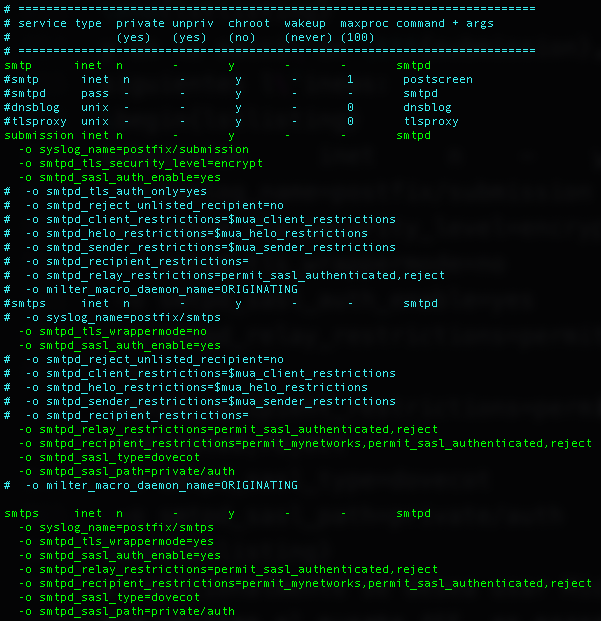
\includegraphics[width=0.75\textwidth]{email/postfixSub}
  \caption{Configuraci\'on del servicio de env\'io de Postfix.}
  \label{fig:email-postfixSub}
\end{figure}

A continuaci\'on, tenemos que especificar a Postfix
el lugar donde se encuentra nuestro certificado de
seguridad y llave privada.   Para abrir el archivo
de configuraci\'on, ejecutamos el comando
\begin{lstlisting}
sudo vi /etc/postfix/main.cf
\end{lstlisting}
y modificamos las l\'ineas relativas a la ubicaci\'on
del certificado y llave TLS como en la Figura
\ref{fig:email-tlsLocation}

\begin{figure}[H]
  \centering
  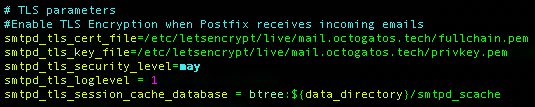
\includegraphics[width=0.75\textwidth]{email/tlsLocation}
  \caption{Configuraci\'on del certificado TLS para Postfix.}
  \label{fig:email-tlsLocation}
\end{figure}

Ahora es posible instalar
\href{https://www.dovecot.org/}{Dovecot} con el
siguiente comando
\begin{lstlisting}
$ sudo apt install dovecot-lmtpd
\end{lstlisting}
y ajustar la configuraci\'on principal con
el comando
\begin{lstlisting}
$ sudo vi /etc/dovecot/dovecot.conf
\end{lstlisting}
donde tenemos que agregar \ttt{lmtp} y \ttt{pop3}
a los protocolos aceptados.

Adem\'as, se debe modificar el siguiente archivo
\begin{lstlisting}
sudo vi /etc/dovecot/conf.d/10-master.conf
\end{lstlisting}
para ajustar la definici\'on del servicio \ttt{lmtp},
para que quede como en la Figura \ref{fig:email-lmtp}.

\begin{figure}[H]
  \centering
  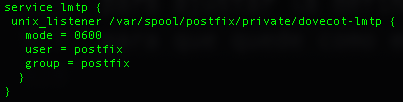
\includegraphics[width=0.75\textwidth]{email/lmtp}
  \caption{Configuraci\'on del servicio lmtp de Dovecot.}
  \label{fig:email-lmtp}
\end{figure}

Para terminar, es necesario indicar a Postfix que
entregue los mensajes al almacenamiento local,
mediante el servidor LMTP de Dovecot.   Esto se
hace en la configuraci\'on principal de Postfix
\begin{lstlisting}
sudo vi /etc/postfix/main.cf
\end{lstlisting}
agregando las siguientes dos l\'ineas al final
del archivo
\begin{lstlisting}
mailbox_transport = lmtp:unix:private/dovecot-lmtp
smtputf8_enable = no
\end{lstlisting}

\begin{figure}[H]
  \centering
  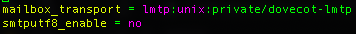
\includegraphics[width=0.75\textwidth]{email/lmtp2}
  \caption{Uso del servicio lmtp de Dovecot en Postfix.}
  \label{fig:email-lmtp2}
\end{figure}

Finalmente, reiniciamos Postfix y Dovecot con
el comando
\begin{lstlisting}
sudo systemctl restart postfix dovecot
\end{lstlisting}

En este momento, es posible configurar un cliente
de correo, como Thunderbird.   Una posible
configuraci\'on del servidor de entrada se
muestra en la Figura \ref{fig:email-tbirdout}
y una posible configuraci\'on del servidor
de salida en la Figura \ref{fig:email-tbirdout}.

\begin{figure}[H]
  \centering
  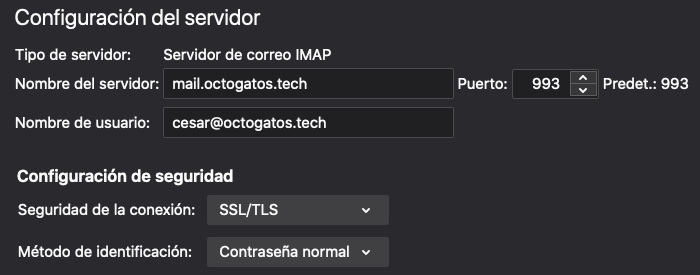
\includegraphics[width=0.75\textwidth]{email/tbirdin}
  \caption{Configuraci\'on del servidor IMAPS para
           usar Thunderbird con nuestro servidor de correo.}
  \label{fig:email-tbirdin}
\end{figure}

\begin{figure}[H]
  \centering
  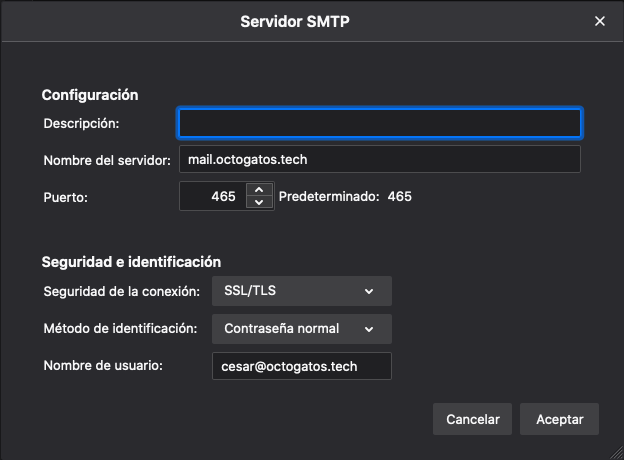
\includegraphics[width=0.75\textwidth]{email/tbirdout}
  \caption{Configuraci\'on del servidor SMTPS para
           usar Thunderbird con nuestro servidor de correo.}
  \label{fig:email-tbirdout}
\end{figure}

En la Figura \ref{fig:email-tbird} se muestra evidencia
del funcionamiento de la configuraci\'on.   Se tiene un
correo en la bandeja entrada de \ttt{cesar@octogatos.tech}
enviado por \ttt{cesar@octogatos.tech}.

\begin{figure}[H]
  \centering
  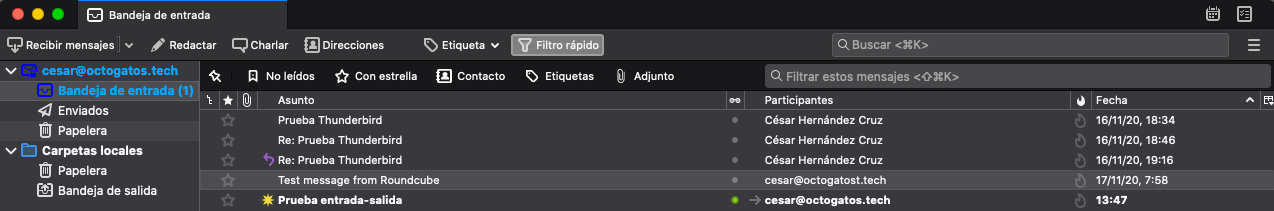
\includegraphics[width=0.9\textwidth]{email/tbird}
  \caption{Bandeja de entrada de \ttt{cesar@octogatos.tech}.}
  \label{fig:email-tbird}
\end{figure}

Aunque en este punto el servidor de correo ya funciona,
s\'olo funciona con cuentas locales de Linux, es decir,
con cuentas creadas directamente en el servidor.   El
siguiente paso es crear buzones virtuales para poder
asignar cuentas a usuarios que no necesariamente tienen
una cuenta en el servidor.    El primer paso ser\'a
crear una pila LAMP (Linux, Apache, MariaDB, PHP),
para lo cu\'al referimos al lector al siguiente
\href{https://www.linuxbabe.com/ubuntu/install-lamp-stack-ubuntu-20-04-server-desktop}{tutorial}.   La finalidad
de esta pila de aplicaciones ser\'a tener un ambiente
en el que podamos crear los buzones virtuales; como
su nombre lo indica, el sistema operativo es Linux,
el servidor web es Apache, la base de datos es
MariaDB, y el lenguaje responsable de generar p\'aginas
web din\'amicas en el servidor es PHP.

Para la creaci\'on y manejo de buzones virtuales
utilizaremos
\href{http://postfixadmin.sourceforge.net/}{PostfixAdmin},
una interfaz web para configurar y administrar un servidor
de correo en Postfix para m\'ultiples usuarios.

En nuestro caso utilizamos MariaDB, pero en caso de
que se est\'e utilizando MySQL, se puede instalar
el paquete \ttt{dbconfig-no-thanks} para evitar que
la instalaci\'on de PostfixAdmin intente configurar
la base de datos.   Esto se puede hacer con el comando
\begin{lstlisting}
$ sudo apt install dbconfig-no-thanks
\end{lstlisting}
tras lo cu\'al es posible instalar PostfixAdmin
\begin{lstlisting}
$ sudo apt install postfixadmin
\end{lstlisting}
remover el paquete antes referido
\begin{lstlisting}
$ sudo apt remove dbconfig-no-thanks
\end{lstlisting}
y finalmente, configurar la base de datos
\begin{lstlisting}
$ sudo dpkg-reconfigure postfixadmin
\end{lstlisting}

Las opciones que deben elegirse son
$\ttt{mysql} \to \ttt{Unix socket} \to
 \ttt{default} \to \ttt{postfixadmin} \to
 \ttt{postfixadmin@localhost}$, tras lo
cu\'al se elige un password y nombre de
usuario para el administrador.   Tras
esta acci\'on, es necesario modificar
dos archivos de configuraci\'on de
PostfixAdmin.   Primero
\begin{lstlisting}
$ sudo vi /etc/dbconfig-common/postfixadmin.conf
\end{lstlisting}
donde se debe cambiar la l\'inea
\begin{lstlisting}
dbc_dbtype='mysql'
\end{lstlisting}
por
\begin{lstlisting}
dbc_dbtype='mysqli'
\end{lstlisting}

Adem\'as
\begin{lstlisting}
$ sudo vi /etc/postfixadmin/dbconfig.inc.php
\end{lstlisting}
donde la l\'inea
\begin{lstlisting}
$dbtype='mysql';
\end{lstlisting}
se cambia por \begin{lstlisting}
$dbtype='mysqli';
\end{lstlisting}

Adem\'as, es necesario crear un directorio
donde estar\'an los templates de PostfixAdmin,
y brindarle los permisos necesarios a
\ttt{www-data} para leer, escribir y ejecutar
en este directorio.
\begin{lstlisting}
$ sudo mkdir /usr/share/postfixadmin/templates_c

$ sudo setfacl -R -m u:www-data:rwx /usr/share/postfixadmin/templates_c/
\end{lstlisting}

Ahora podemos crear un virtual host para
PostfixAdmin.  Es necesario crear el archivo
para la configuraci\'on correspondiente con
el comando
\begin{lstlisting}
sudo vi /etc/apache2/sites-available/postfixadmin.conf
\end{lstlisting}
el contenido de dicho archivo debe verse como
en la Figura \ref{fig:email-vhost}

\begin{figure}[H]
  \centering
  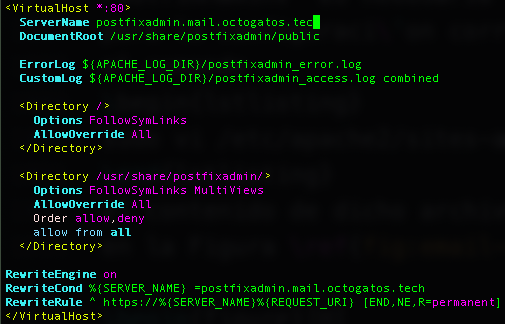
\includegraphics[width=0.9\textwidth]{email/vhost}
  \caption{Configuraci\'on del virtual host para PostfixAdmin.}
  \label{fig:email-vhost}
\end{figure}

Para activar la configuraci\'on, es necesario
ejecutar los comandos
\begin{lstlisting}
$ sudo a2ensite postfixadmin.conf

$ sudo systemctl reload apache2
\end{lstlisting}

Ahora es posible ejecutar el install-wizard de
PostfixAdmin desde \href{http://postfixadmin.octogatos.tech/setup.php}{http://postfixadmin.octogatos.tech/setup.php}
(actualmente el v\'inculo est\'a desactivado, pues
ya concluy\'o la instalaci\'on).

El siguiente paso es instalar alg\'unos m\'odulos
de PHP requeridos o recomendados por PostfixAdmin.
\begin{lstlisting}
$ sudo apt install php7.4-fpm php7.4-imap php7.4-mbstring php7.4-mysql php7.4-json php7.4-curl php7.4-zip php7.4-xml php7.4-bz2 php7.4-intl php7.4-gmp
\end{lstlisting}

La encriptaci\'on que Dovecot usa por omisi\'on
es \ttt{MD5-CRYPT}, que no es muy segura.  La cambiaremos
a una m\'as segura, \ttt{ARGON2I}.   Para esto,
abrimos el archivo de configuraci\'on local de
PostfixAdmin
\begin{lstlisting}
$ sudo vi /usr/share/postfixadmin/config.local.php
\end{lstlisting}
y agregamos las l\'ineas que se muestran en la
Figura \ref{fig:email-argon}.

\begin{figure}[H]
  \centering
  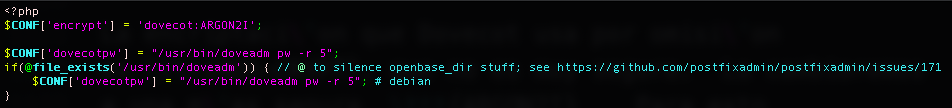
\includegraphics[width=0.9\textwidth]{email/argon}
  \caption{Configuraci\'on del esquema de encriptaci\'on.}
  \label{fig:email-argon}
\end{figure}
Finalmente, terminamos la instalaci\'on en nuestro
navegador en la direcci\'on
\ttt{postfixadmin.octogatos.teh/setup.php} (ahora
deshabilitada).   Tras crear el hash de la contrase\~na,
es necesario modificar el archivo \\
\ttt{/usr/share/postfixadmin/config.local.php}, agregando
la l\'inea final con nuestro hash.   El resultado final
puede verse en la Figura \ref{fig:email-hash}.
\begin{figure}[H]
  \centering
  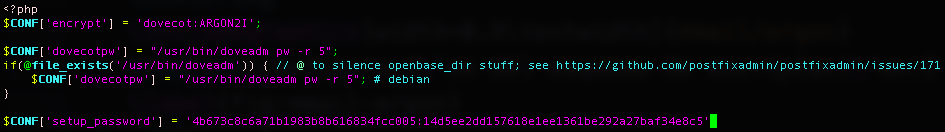
\includegraphics[width=0.9\textwidth]{email/hash}
  \caption{Agregando el hash de la contrase\~na para el
           administrador en PostfixAdmin.}
  \label{fig:email-hash}
\end{figure}

Ahora es posible ingresar a la aplicaci\'on web
mediante
\href{https://postfixadmin.mail.octogatos.tech/login.php}{esta direcci\'on}, como se observa en la Figura
\ref{fig:email-postfixAdmin}.
\begin{figure}[H]
  \centering
  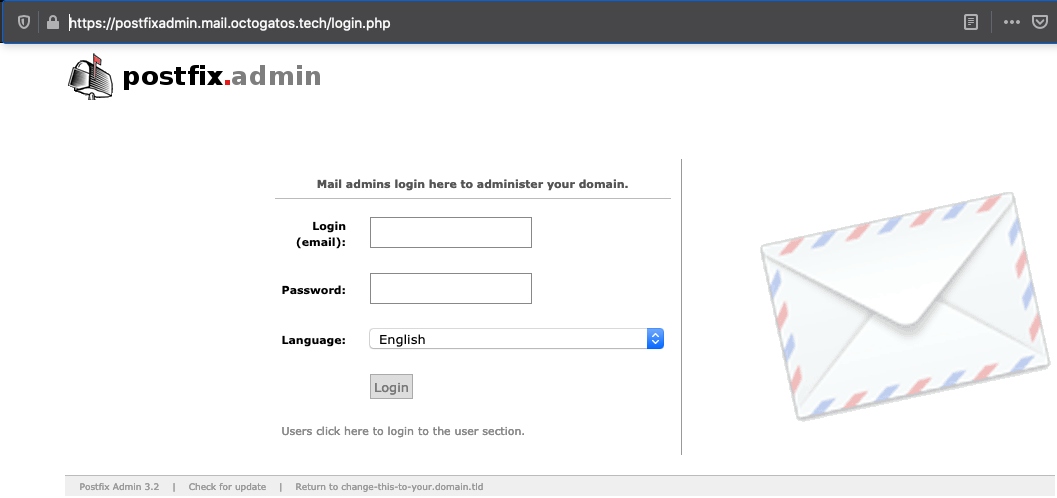
\includegraphics[width=0.9\textwidth]{email/postfixAdmin}
  \caption{Aplicaci\'on PostfixAdmin corriendo en nuestro
           servidor.}
  \label{fig:email-postfixAdmin}
\end{figure}

El siguiente paso es configurar Postfix y Dovecot para
usar MariaDB, los pasos son sencillos, pero t\'ecnicos y
tediosos, por lo que simplemente referimos al lector
a la \href{https://www.linuxbabe.com/mail-server/postfixadmin-create-virtual-mailboxes-ubuntu-20-04}{siguiente liga}.
Tras realizar esta configuraci\'on, es posible cerar
buzones virtuales para nuevos usuarios de correo en
la p\'agina de PostfixAdmin.   M\'as importante, es
posible configurar un cliente de email web para tener
acceso a nuestro servidor de correo.   Utilizamos
\href{https://roundcube.net/}{Roundcube} y seguimos
\href{https://www.linuxbabe.com/ubuntu/install-roundcube-webmail-ubuntu-20-04-apache-nginx}{este tutorial} para
configurarlo.  El resultado final puede observarse
en \href{https://mail.octogatos.tech}{mail.octogatos.tech},
y la Figura \ref{fig:email-roundcube} muestra la aplicac\'on
en funcionamiento.
\begin{figure}[H]
  \centering
  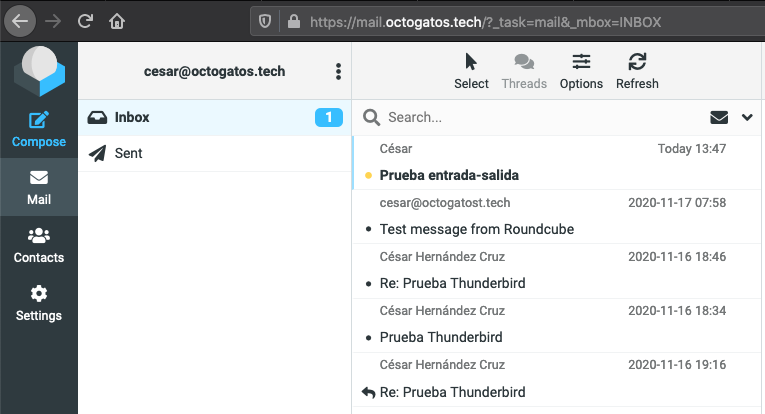
\includegraphics[width=0.9\textwidth]{email/roundcube}
  \caption{Aplicaci\'on Roundcube corriendo en nuestro
           servidor.}
  \label{fig:email-roundcube}
\end{figure}


Finalmente, configuramos los registros SPF, DKIM y DMARC.
La correcta configuraci\'on de estos registros redundar\'a
en que nuestro servidor no pueda ser utilizado por terceros
para enviar correos, es decir, no est\'a en open relay.

La configuraci\'on del registro SPF es muy sencilla, basta
con seguir el formato de la Figura \ref{fig:email-spf}.
\begin{figure}[H]
  \centering
  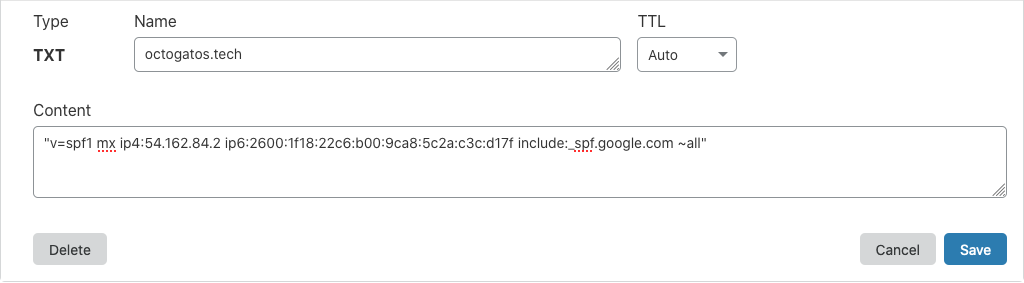
\includegraphics[width=0.9\textwidth]{email/spf}
  \caption{Configuraci\'on de registro SPF.}
  \label{fig:email-spf}
\end{figure}

La configuraci\'on del registro DKIM es un poco m\'as
elaborada.   Utilizamos \href{http://opendkim.org/}{OpenDKIM}
para configurarlo en nuestro servidor, y crear la llave
p\'ublica cuyo hash se integr\'o al registro
correspondiente.   Nuevamente, la configuraci\'on
es sencilla, pero larga y t\'ecnica, por lo que
simplemente referimos al lector a
\href{https://www.linuxbabe.com/mail-server/setting-up-dkim-and-spf}{este tutorial}. Una vez configurada esta
aplicaci\'on, es necesario crear un par de
llave p\'ublica y privada, para lo cu\'al es
necesario crear primero una carpeta para nuestro
dominio
\begin{lstlisting}
sudo mkdir /etc/opendkim/keys/octogatos.tech
\end{lstlisting}
generar las llaves
\begin{lstlisting}
sudo opendkim-genkey -b 2048 -d octogatos.tech -D /etc/opendkim/keys/octogatos.tech -s default -v
\end{lstlisting}
hacer a OpenDKIM el due\~no de la llave privada
\begin{lstlisting}
sudo chown opendkim:opendkim /etc/opendkim/keys/octogatos.tech/default.private
\end{lstlisting}
y finalmente publicar la llave p\'ublica en el registro
DKIM correspondiente.   Es posible acceder al archivo
donde se encuentra el hash de la llave p\'ublica con
el comando
\begin{lstlisting}
sudo cat /etc/opendkim/keys/octogatos.tech/default.txt
\end{lstlisting}
como se muestra en la Figura \ref{fig:email-hashdkim}.

\begin{figure}[H]
  \centering
  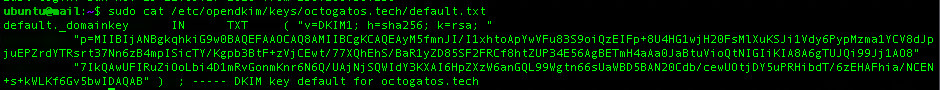
\includegraphics[width=0.9\textwidth]{email/hashdkim}
  \caption{Obtenci\'on del hash de la llave p\'ublica para
           el registro DKIM.}
  \label{fig:email-hashdkim}
\end{figure}

Con esta informaci\'on, es ahora posible configurar el
registro DKIM como se muestra en la Figura
\ref{fig:email-dkim}

\begin{figure}[H]
  \centering
  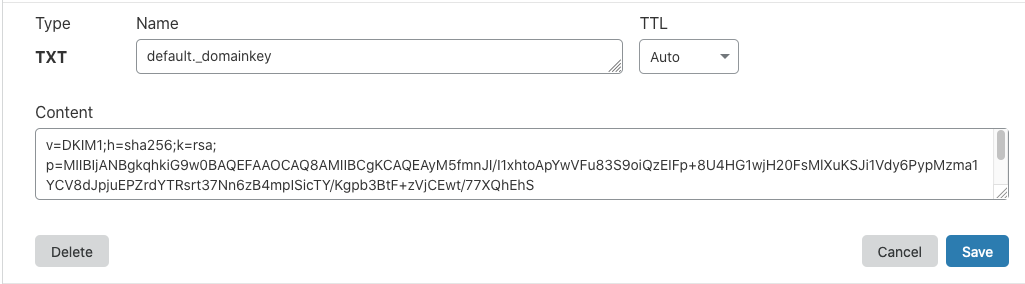
\includegraphics[width=0.9\textwidth]{email/dkim}
  \caption{Configuraci\'on del registro DKIM.}
  \label{fig:email-dkim}
\end{figure}

Una vez con ambos registros configurados, la configuraci\'on
del registro DMARC se reduce a crear el registro como se
muestra en la Figura \ref{fig:email-dmarc}.

\begin{figure}[H]
  \centering
  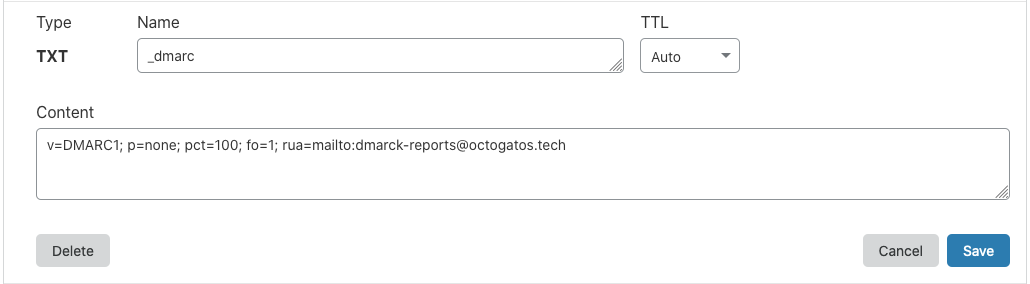
\includegraphics[width=0.9\textwidth]{email/dmarc}
  \caption{Configuraci\'on del registro DMARC.}
  \label{fig:email-dmarc}
\end{figure}

Hay varias formas de verificar que estas configuraciones
fueron correctas, una sencilla es enviar un corro desde
nuestro servidor a cualquier direcci\'on de correo
manejada por Google, y ver los detalles en ``Mostrar
mensaje original'', donde podemos ver las entradas
mostradas en la Figura \ref{fig:email-spfdkimdmarc}.

\begin{figure}[H]
  \centering
  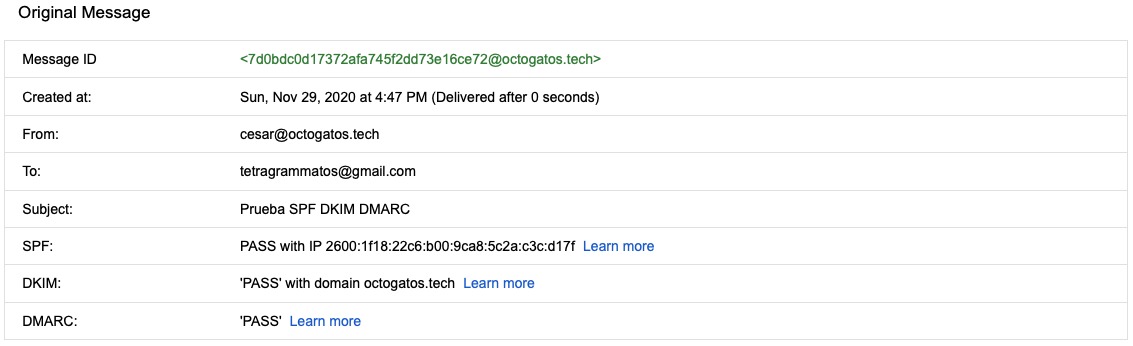
\includegraphics[width=0.9\textwidth]{email/spfdkimdmarc}
  \caption{Verificaci\'on de la configuraci\'on de los
           registros SPF, DKIM y DMARC.}
  \label{fig:email-spfdkimdmarc}
\end{figure}

La correcta configuraci\'on de estos tres registros,
junto con el registro PTR de DNS, que se realiz\'o
mediante una solicitud a AWS, impide que nuestro
servidor sea utilizado para que terceros no autorizados
env\'ien correo a trav\'es de nuestro servidor.   En
otras palabras, nuestro servidor no est\'a en open relay.

Para evaluar la funcionalidad de nuestro servidor de
correo, por favor manden un correo a
\ttt{cesar@octogatos.tech}.

Una evaluaci\'on en l\'inea de nuestro servidor arroj\'o
los resultados que aparecen en la Figura \ref{fig:email-test}.

\begin{figure}[H]
  \centering
  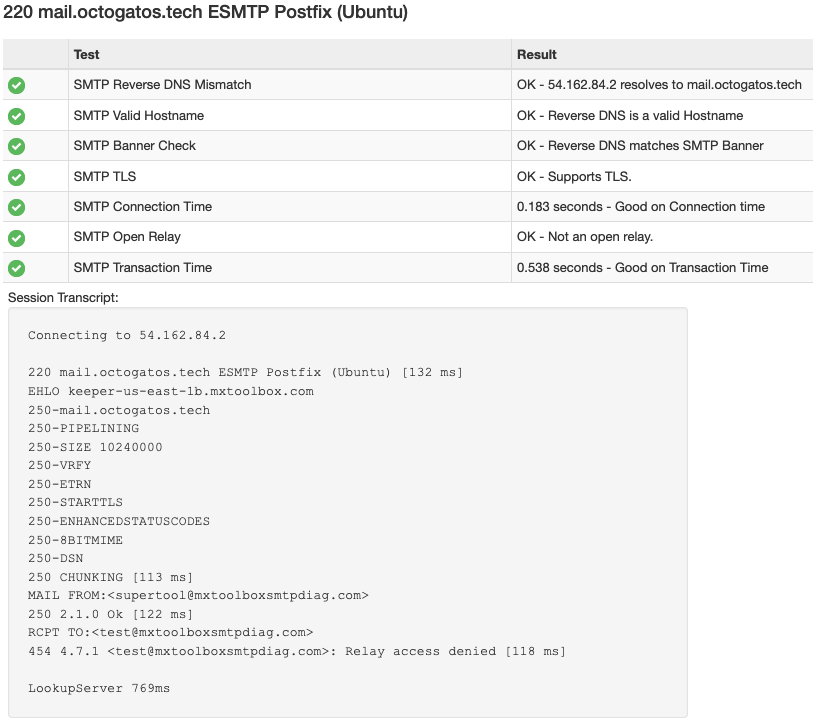
\includegraphics[width=0.75\textwidth]{email/test}
  \caption{Prueba con \href{https://mxtoolbox.com/diagnostic.aspx}{https://mxtoolbox.com/diagnostic.aspx}.}
  \label{fig:email-test}
\end{figure}


%%%%%%%%%%%%%%%%%%%%%%%%%%%%%%%%%%%%%%%%%%%%%%%%%%%%%%%%%%%%%%%%
%%%%%%%%%%%%%%%%%%%%%%%%%%%%%%%%%%%%%%%%%%%%%%%%%%%%%%%%%%%%%%%%
%%%%%%%%%%%%%%%%%%%%%%%%%%%%%%%%%%%%%%%%%%%%%%%%%%%%%%%%%%%%%%%%
%%%%%%%%%%%%%%%%%%%%%%%%               %%%%%%%%%%%%%%%%%%%%%%%%%
%%%%%%%%%%%%%%%%%%%%%%%%%%%%%%%%%%%%%%%%%%%%%%%%%%%%%%%%%%%%%%%%
%%%%%%%%%%%%%%%%%%%%%%%%%%%%%%%%%%%%%%%%%%%%%%%%%%%%%%%%%%%%%%%%
%%%%%%%%%%%%%%%%%%%%%%%%%%%%%%%%%%%%%%%%%%%%%%%%%%%%%%%%%%%%%%%%


\section{Configuraci\'on NAT}

Como se puede ver en la Secci\'on \ref{sec:diagrama},
se crearon dos subredes p\'ublicas y una privada, con
un NAT gateway configurado dentro de una de las subredes
p\'ublicas.   A continuaci\'on describimos c\'omo se
llev\'o a cabo dicha configuraci\'on; el punto
principal es que las instancias que corren en la subred
privada no tienen una direcci\'on IP p\'ublica, por lo
que no pueden ser accedidas desde el exterior de la VPC.
Para conectarnos a \'estas, utilizamos su direcci\'on
IP privada desde las instancias que se encuentran corriendo
en las subredes p\'ublicas.

Como prerrequisitos, consideramos que ya existen las
dos instancias EC2 p\'ublicas corriendo y que est\'an
cada una en una red con la configuraci\'on por omisi\'on,
con la VPC por omisi\'on, y la Route Table por omisi\'on.

La configuraci\'on de estas subredes, que se
utilizar\'an como subredes p\'ublicas, se muestran en las
Figuras \ref{fig:NAT-webSubnet} y \ref{fig:NAT-emailSubnet}.
Adem\'as de la explicaci\'on brindada por el profesor en
Discord, nos apoyamos en el siguiente documento de AWS.
\href{https://docs.aws.amazon.com/vpc/latest/userguide/VPC_Scenario2.html}{https://docs.aws.amazon.com/vpc/latest/userguide/VPC\_Scenario2.html}

\begin{figure}[H]
  \centering
  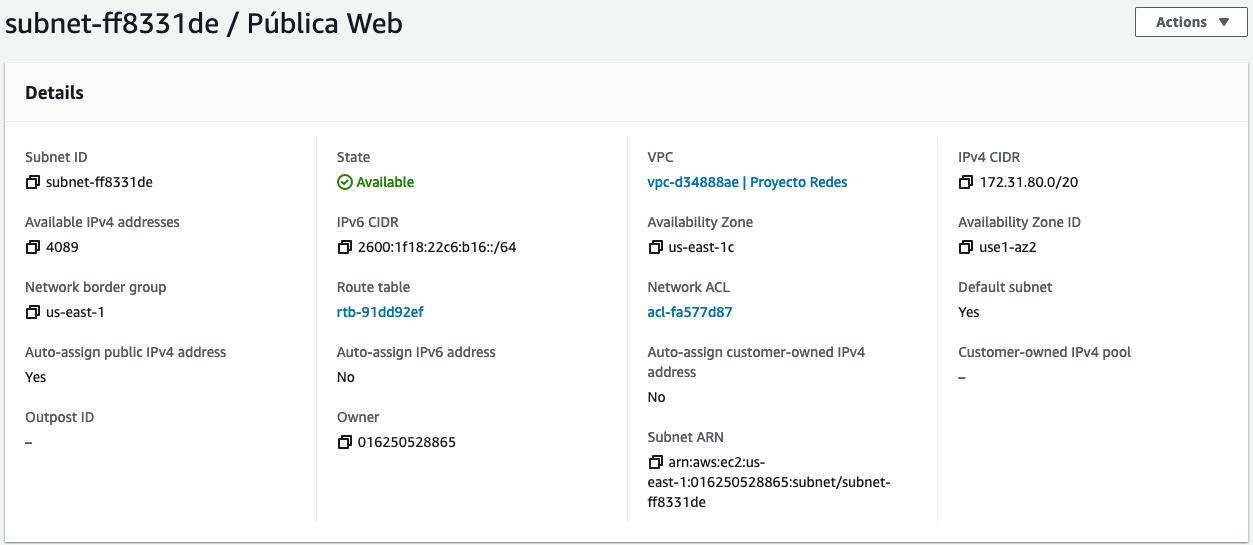
\includegraphics[width=\textwidth]{NAT/webSubnet}
  \caption{Configuraci\'on de la subred p\'ublica del
           servidor web.}
  \label{fig:NAT-webSubnet}
\end{figure}

\begin{figure}[H]
  \centering
  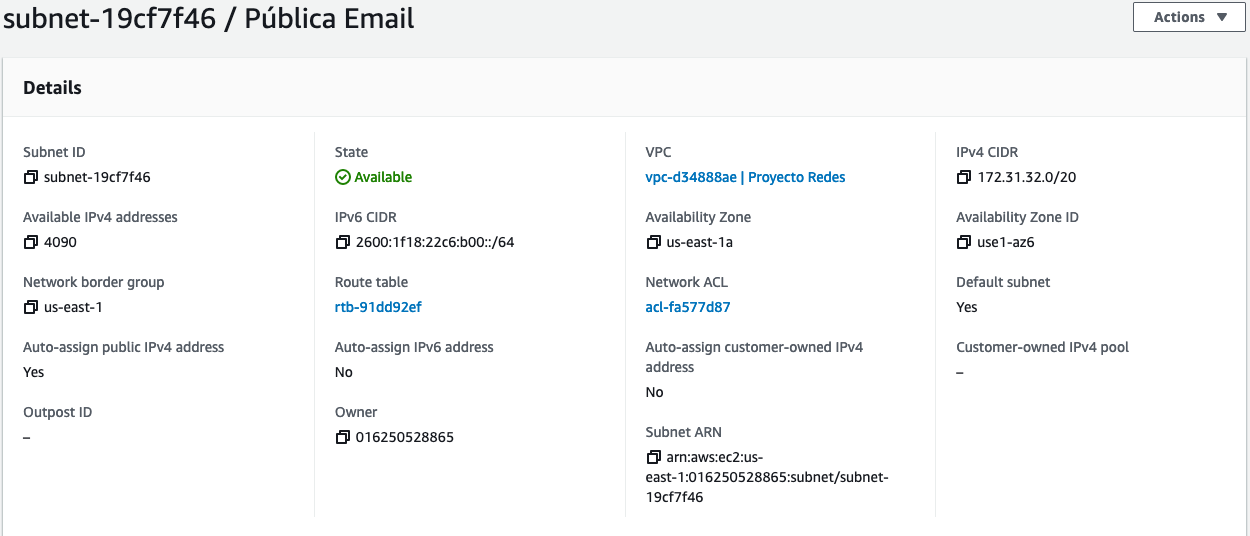
\includegraphics[width=\textwidth]{NAT/emailSubnet}
  \caption{Configuraci\'on de la subred p\'ublica del
           servidor web.}
  \label{fig:NAT-emailSubnet}
\end{figure}

\begin{enumerate}
  \item Creamos una nueva subred, en la misma zona de
    disponibilidad que la red que ya ten\'iamos, y con
    conjunto de direcciones IPv4 en el mismo segmento
    que la anterior.   En la captura de pantalla hay un
    error, hab\'iamos nombrado ``P\'ublica'' a esta red,
    pero esta realmente es la privada (el error se
    corrigi\'o posteriormente).    La configuraci\'on
    puede verse en la Figura \ref{fig:NAT-priSubnet}. Una
    observaci\'on importante es que se deshabilit\'o
    la opci\'on de asignar autom\'aticamente una
    direcci\'on IPv4 a las instancias que se creen
    dentro de esta subred.   Adem\'as de la explicaci\'on
    compartida por el profesor, nos apoyamos en el
    siguiente documento de AWS: \href{https://docs.aws.amazon.com/cloudhsm/latest/userguide/create-subnets.html}{https://docs.aws.amazon.com/cloudhsm/latest/userguide/create-subnets.html}.
    \begin{figure}[H]
      \centering
      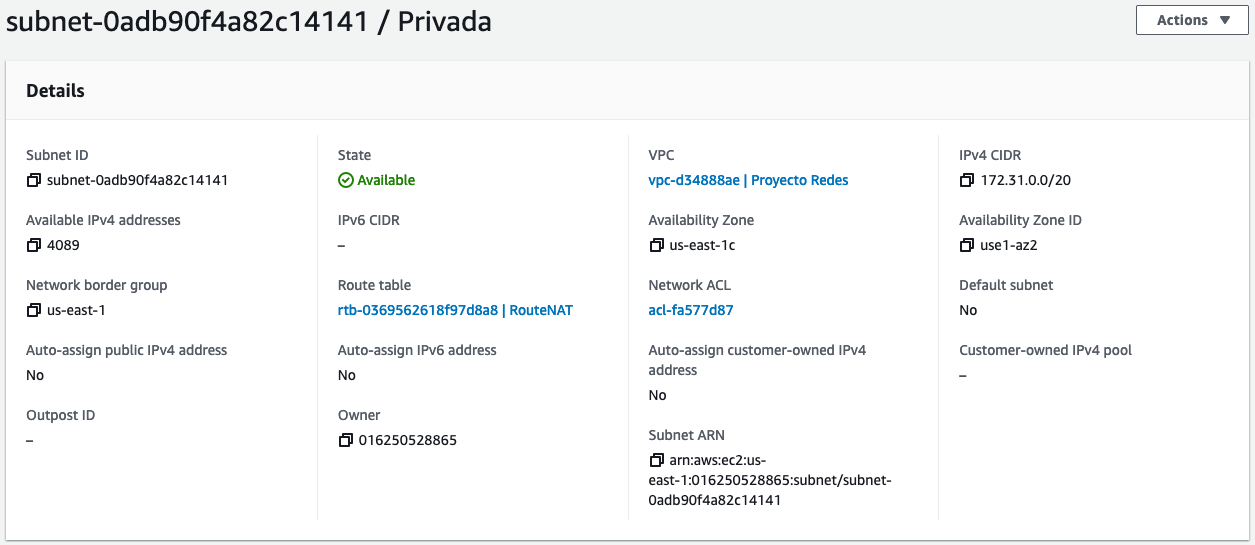
\includegraphics[width=0.8\textwidth]{NAT/privateSubnet}
      \caption{Configuraci\'on de la subred privada.}
      \label{fig:NAT-priSubnet}
    \end{figure}

  \item Posteriormente, creamos dos nuevas instancias,
    en la misma \'area de disponibilidad que la instancia
    correspondiente al servidor web, pero en la subred
    privada reci\'en creada. La configuraci\'on de estas
    instancias puede verse en las Figuras
    \ref{fig:NAT-appInstance} y \ref{fig:NAT-dataInstance}.
    Es importante hacer notar que estas instancias no cuentan
    con una direcciones IPv4 p\'ublicas.
    \begin{figure}[H]
      \centering
      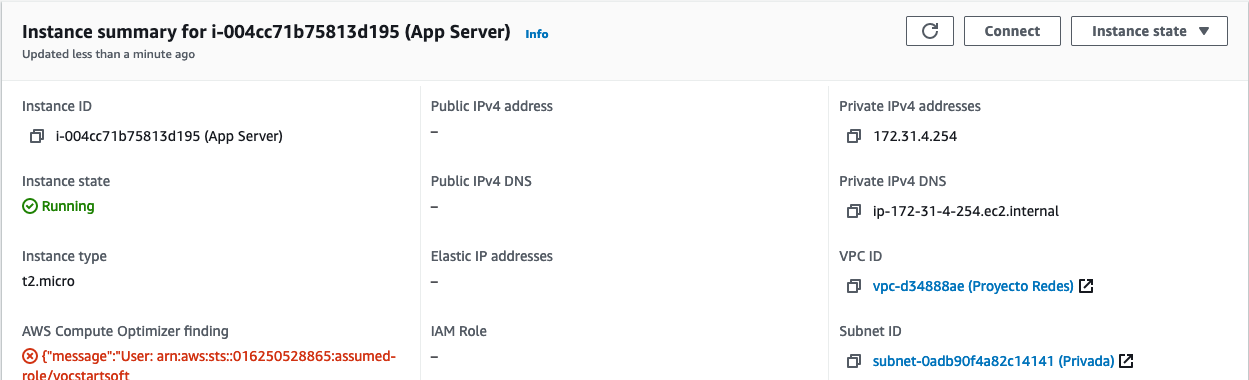
\includegraphics[width=\textwidth]{NAT/appInstance}
      \caption{Configuraci\'on de la instancia correspondiente
               al app server.}
      \label{fig:NAT-appInstance}
    \end{figure}

    \begin{figure}[H]
      \centering
      \includegraphics[width=\textwidth]{NAT/dataInstance}
      \caption{Configuraci\'on de la instancia correspondiente
               al data server.}
      \label{fig:NAT-dataInstance}
    \end{figure}

  \item El siguiente paso fue crear el NAT gateway.   La
    configuraci\'on resultante aparece en la Figura
    \ref{fig:NAT-nat}.  Cabe resaltar la importancia de
    asignar una IP el\'astica al NAT gateway al momento
    de crearlo. Nos apoyamos en las instrucciones que el
    profesor comparti\'o en Discord y el siguiente
    documento de AWS:
    \href{https://aws.amazon.com/premiumsupport/knowledge-center/nat-gateway-vpc-private-subnet/}{https://aws.amazon.com/premiumsupport/knowledge-center/nat-gateway-vpc-private-subnet/}
    \begin{figure}[H]
      \centering
      \includegraphics[width=\textwidth]{NAT/nat}
      \caption{Configuraci\'on del NAT gateway.}
      \label{fig:NAT-nat}
    \end{figure}

  \item Posteriormente, creamos una nueva tabla de
    ruteo.   Es necesario agregar una ruta, con destino
    \ttt{0.0.0.0/0} y target el NAT gateway reci\'en
    creado.   La configuraci\'on resultante puede
    verse en la Figura \ref{fig:NAT-routeTable}.
    \begin{figure}[H]
      \centering
      \includegraphics[width=\textwidth]{NAT/routeTable}
      \caption{Configuraci\'on de la nueva tabla de ruteo.}
      \label{fig:NAT-routeTable}
    \end{figure}

  \item Para terminar, asociamos la subred privada con
    la tabla de ruteo creada en el paso anterior. El
    resultado de esa asociaci\'on se observa en la Figura
    \ref{fig:subnetRouteTable}.
    \begin{figure}[H]
      \centering
      \includegraphics[width=\textwidth]{NAT/subnetRouteTable}
      \caption{Subred privada asociada a la nueva tabla
      de ruteo.}
      \label{fig:subnetRouteTable}
    \end{figure}
\end{enumerate}

Una vez terminada la configuraci\'on, podemos verificar
que funcione correctamente con los siguientes pasos.

\begin{enumerate}
  \item Ingresar a la instancia p\'ublica, con el
    comando
\begin{lstlisting}
$ ssh -i "practica2.pem" ssh -i "practica2.pem" ubuntu@ec2-52-87-39-6.compute-1.amazonaws.com
\end{lstlisting}

  \item Una vez dentro de alguna de las instancias p\'ublicas
    (en el ejemplo el servidor web) ingresar a alguna de las
    privadas (en el ejemplo el servidor de aplicaci\'on)
    mediante su direcci\'on IP privada, o en
    nuestro caso con su nombre de dominio privado,
    previamente configurado con Route 53, con el comando
\begin{lstlisting}
$ ssh -i "practica2.pem" ubuntu@app.octogatos.tech
\end{lstlisting}

  \item Verificar la conectividad a internet, por
    ejemplo, con un ping a google.com
\begin{lstlisting}
$ ping google.com
\end{lstlisting}

  \item Al no contar con direcci\'on IP p\'ublica
    ni siquiera es posible intentar conectarnos a
    la instancia privada externamente, pues su
    direcci\'on IP privada, as\'i como su nombre
    de dominio privado, son relativos a la VPC.
\end{enumerate}

\begin{figure}[H]
  \centering
  \includegraphics[width=\textwidth]{NAT/result}
  \caption{Subred privada asociada a la nueva tabla
  de ruteo.}
  \label{fig:NAT-result}
\end{figure}

El resultado de los pasos antes descritos puede
revisarse en la Figura \ref{fig:NAT-result}.
\begin{figure}[H]
  \centering
  \includegraphics[width=0.35\textwidth]{NAT/inception}
  \caption{It's like inception!}
\end{figure}

\section{FAIL2BAN}

Como nuestros servidores son servicios que se encuentran
disponibles en el internet, estos son vulnerables a
ataques maliciosos; por ello los tenemos que proteger para
que a su vez podamos proteger a nuestro usuarios.

En esta ocasión se hizo uso de la herramienta \ttt{FAIL2BAN}
que nos permite detectar ataques maliciosos automatizados
como fuerza bruta u otros, detectando las direcciones IP
de las que provienen estos ataques y baneandolos en el
intento, rechazando cualquier futura conexión o petición
de ellos por un tiempo definido.

Se procedió entonces a instalar \ttt{FAIL2BAN} en todos
nuestros servidores, y se dejaron las configuraciones por
omisión de esta instalación.

\begin{figure}[H]
  \centering
  \includegraphics[width=0.35\textwidth]{FAIL2BAN/exhibitB}
  \caption{Servicio FAIL2BAN corriendo en el Web Server}
\end{figure}

\begin{figure}[H]
  \centering
  \includegraphics[width=0.35\textwidth]{FAIL2BAN/exhibitD}
  \caption{Servicio FAIL2BAN corriendo en el Mail Server}
\end{figure}

\begin{figure}[H]
  \centering
  \includegraphics[width=0.35\textwidth]{FAIL2BAN/exhibitA}
  \caption{Servicio FAIL2BAN corriendo en el App Server}
\end{figure}

\begin{figure}[H]
  \centering
  \includegraphics[width=0.35\textwidth]{FAIL2BAN/exhibitC}
  \caption{Servicio FAIL2BAN corriendo en el Data Server}
\end{figure}

\section{Comentarios sobre el desarrollo del proyecto}

En general, nos enfrentamos a las dificultades propias
de un proyecto de este tipo; por suerte no tuvimos
contratiempos m\'as all\'a de problemas de configuraci\'on,
que finalmente fueron arreglados.   Sin embargo, en gran
medida las cosas funcionaron bien gracias a que un
integrante del equipo (Mauricio Carrasco) ten\'ia 100
cr\'editos de AWS, de otro modo, no hubi\'eramos conseguido
realizar la configuraci\'on completa con 30 cr\'editos.

Estamos muy contentos de haber podido hacer el proyecto
completo como se plante\'o orignalmente, pues nos permiti\'o
ver el funcionamiento en conjunto, y la utilidad de cada
una de las componentes de la configuraci\'on de nuestro
servicio.   Este desarrollo nos brind\'o una idea general
de c\'omo funciona un servicio de este tipo en la vida
real, principalmente sobre todas las decisiones que se
pueden tomar para hacer la configuraci\'on (y agradecemos
que ustedes hayan tomado la mayor parte de las decisiones
por nosotros).

Una nota importante sobre las referencias t\'ecnicas.
Decidimos incluir las referencias t\'ecnicas en el cuerpo
del texto, como hiperv\'inculos en los lugares donde la
informaci\'on correspondiente resulta relevante.   Por
esta raz\'on, no tenemos una secci\'on especial para
las referencias t\'ecnicas.

Respecto a este documento, una nota importante es que,
aunque algunas im\'agenes tienen un tama\~no reducido,
por motivos de formato, la mayor\'ia de ellas tienen
una resoluci\'on bastante alta, por lo que es posible
examinarlas haciendo zoom sobre ellas.

\end{document}
